%% LyX 1.6.7 created this file.  For more info, see http://www.lyx.org/.
%% Do not edit unless you really know what you are doing.
\documentclass[english]{article}
\usepackage[T1]{fontenc}
\usepackage[latin9]{inputenc}
\usepackage[letterpaper]{geometry}
\geometry{verbose,tmargin=1in,bmargin=1in,lmargin=1in,rmargin=1in}
\setcounter{tocdepth}{1}
\usepackage{babel}

\usepackage{float}
\usepackage{textcomp}
\usepackage{amsmath}
\usepackage{graphicx}
\usepackage{amssymb}
\usepackage[unicode=true, pdfusetitle,
 bookmarks=true,bookmarksnumbered=false,bookmarksopen=false,
 breaklinks=true,pdfborder={0 0 0},backref=false,colorlinks=false]
 {hyperref}

\makeatletter

%%%%%%%%%%%%%%%%%%%%%%%%%%%%%% LyX specific LaTeX commands.
\providecommand{\LyX}{L\kern-.1667em\lower.25em\hbox{Y}\kern-.125emX\@}
\newcommand{\lyxmathsym}[1]{\ifmmode\begingroup\def\b@ld{bold}
  \text{\ifx\math@version\b@ld\bfseries\fi#1}\endgroup\else#1\fi}

%% Special footnote code from the package 'stblftnt.sty'
%% Author: Robin Fairbairns -- Last revised Dec 13 1996
\let\SF@@footnote\footnote
\def\footnote{\ifx\protect\@typeset@protect
    \expandafter\SF@@footnote
  \else
    \expandafter\SF@gobble@opt
  \fi
}
\expandafter\def\csname SF@gobble@opt \endcsname{\@ifnextchar[%]
  \SF@gobble@twobracket
  \@gobble
}
\edef\SF@gobble@opt{\noexpand\protect
  \expandafter\noexpand\csname SF@gobble@opt \endcsname}
\def\SF@gobble@twobracket[#1]#2{}
%% Because html converters don't know tabularnewline
\providecommand{\tabularnewline}{\\}

%%%%%%%%%%%%%%%%%%%%%%%%%%%%%% User specified LaTeX commands.
\usepackage{clrscode3e}

\makeatother

\begin{document}

\title{Algorithms and Data Structures: notes for UIC qual%
\thanks{This work is licensed under a \underbar{\protect\href{http://creativecommons.org/licenses/by-nc-sa/3.0}{Creative Commons Attribution-NonCommercial-ShareAlike 3.0 Unported License}}.%
}}


\author{Gugo}

\maketitle

\subsection*{Disclaimer}

These notes have been prepared with the \textbf{only} purpose to help
me pass the Computer Science qualifiying exam at the University of
Illinois at Chicago. They are distributed as they are (including errors,
typos, omissions, etc.) to help other students pass this exam (and
possibly relieving them from part of the pain associated with such
a process). I take \textbf{no responsibility} for the material contained
in these notes (which means that you can't sue me if you don't pass
the qual!) Moreover, this pdf version is distributed together with
the original \LaTeX{} (and \LyX{}) sources hoping that someone else
will improve and correct them. I mean in absolute no way to violate
copyrights and/or take credit stealing the work of others. The ideas
contained in these pages are \textbf{not mine} but I've just aggregated
information scattered all over the internet.


\subsection*{Strongly suggested book}

Before you even start reading this notes, do yourself a favor and
go buy the {}``bible of algorithms'' a.k.a. \emph{Introduction to
Algorithms, Third Edition} by Cormen, Laiserson, Rivest, Stein. (\href{http://mitpress.mit.edu/algorithms/}{http://mitpress.mit.edu/algorithms/})
It is very complete and clear. Also, thanks to the authors for the
beautiful \texttt{clrscode3e} package that has been used to write
the pseudocode of all the algorithms in these notes.

\tableofcontents{}

\pagebreak{}

\textbf{Important!!! }Whenever talking about arrays we assume the
index to ALWAYS start at 1 and NOT 0.


\section{Analysis of algorithms%
\footnote{Chapters 2, 3, 4%
}}
\begin{itemize}
\item \textbf{Loop invariants} are useful to demonstrate the correctness
of an algorithm. We need to show they hold during the three execution
phases of an algorithm: \emph{Initialization}, \emph{Maintenance}
and \emph{Termination}. They work similarly to math induction.
\item Goal is to compute the \emph{running time} of an algorithm (on a particular
input!). 
\item Various types of analysis are possible (which running time are we
considering?): worst, best, average. These depend on which input we
are considering.

\begin{itemize}
\item Best case is rarely (never) used because it provides no useful information. 
\item Average case is difficult to guess sometime. 
\item Worst case gives an upper-bound for EVERY input, it occurs fairly
often and often matches the average case.
\end{itemize}
\item Instead of computing just the running time we are interested in the
\emph{order of growth} of the running time. (asymptotic analysis) 
\end{itemize}

\subsection{Asymptotic notation}

Asymptotic notation applies to functions: we describe the running
time of algorithms as a function of the input size $n$ and we then
apply the asymptotic notation to such a function. 


\paragraph{$\mathbf{\Theta}$-notation}

For a given function $g(n)$, we denote $\Theta(g(n))$ the set of
functions \begin{eqnarray*}
\Theta(g(n)) & = & \{(f(n):\text{ there exist positive constants \ensuremath{c_{1}},\ensuremath{c_{2}} and \ensuremath{n_{0}} such that}\\
 &  & 0\leq c_{1}g(n)\leq f(n)\leq c_{2}g(n)\text{ for all }n\geq n_{0}\}\end{eqnarray*}


We write $f(n)=\Theta(g(n))$ to indicate $f(n)\in\Theta(g(n))$ and
say that $g(n)$ is an \emph{asymptotic tight bound} for $f(n)$.


\paragraph{$\mathbf{O}$-notation}

For a given function $g(n)$, we denote $O(g(n))$ the set of functions
\begin{eqnarray*}
O(g(n)) & = & \{(f(n):\text{ there exist positive constants \ensuremath{c} and \ensuremath{n_{0}} such that}\\
 &  & 0\leq f(n)\leq cg(n)\, for\, all\, n\geq n_{0}\}\end{eqnarray*}


We write $f(n)=O(g(n))$ to indicate $f(n)\in O(g(n))$ and say that
$g(n)$ is an \emph{asymptotic upper bound} for $f(n)$.

This notation is important because when we use $O$-notation to describe
the worst-case running time of an algorithm we have a bound on the
running time of the algorithm on \emph{every input}. When we say {}``the
running time of an algorithm is $O(g(n))$'', we mean that there
is a function $f(n)$ that is in $O(g(n))$ such that, no matter what
particular input size $n$ is chosen, the running time on that particular
input is bounded from above by the value $f(n)$.


\paragraph{$\mathbf{\Omega}$-notation}

For a given function $g(n)$, we denote $\Omega(g(n))$ the set of
functions \begin{eqnarray*}
\Omega(g(n)) & = & \{(f(n):\text{ there exist positive constants \ensuremath{c}and \ensuremath{n_{0}} such that}\\
 &  & 0\leq cg(n)\leq f(n)\, for\, all\, n\geq n_{0}\}\end{eqnarray*}


We write $f(n)=\Omega(g(n))$ to indicate $f(n)\in\Omega(g(n))$ and
say that $g(n)$ is an \emph{asymptotic lower bound} for $f(n)$.

When we say {}``the running time of an algorithm is $\Omega(g(n))$'',
we mean that no matter what particular input of size $n$ is chosen
for each value of $n$, the running time on that input is at least
a constant times $g(n)$, for sufficiently large $n$. Equivalently
we are giving a lower bound on the best-case running time of an algorithm.


\subsubsection{Observations}
\begin{itemize}
\item Note that in the definitions of all the previous asymptotic notations
we assumed that every function is \emph{asymptotically nonnegative}
which means that all functions are nonnegative whenever $n$ is sufficiently
large.
\item Note that it is important that we have some choices for the constants.
Therefore if we find just one choice for the constants that is enough
to apply the proper notation. Conversely if we need to show that the
notation is not true we need to show that there is NO choice for the
constants.
\item In polynomials we can generally discard lower order terms when performing
asymptotic analysis because they are insignificant for large $n$.
\item For any two functions $f(n)$ and $g(n)$, we have \[
f(n)=\Theta(g(n))\iff f(n)=O(g(n))\, and\, f(n)=\Omega(g(n))\]

\item Transitivity, reflexivity and symmetry in $\Theta$-notation and transpose
symmetry in $\Omega$-notation and $O$-notation, apply to asymptotic
comparison.
\end{itemize}

\paragraph{$\mathbf{o}$-notation}

For a given function $g(n)$, we denote $o(g(n))$ the set of functions
\begin{eqnarray*}
o(g(n)) & = & \{(f(n)\,:\,\forall c>0,\,\exists n_{0}>0:\\
 &  & 0\leq f(n)<cg(n)\text{ for all }n\geq n_{0}\}\end{eqnarray*}


We write $f(n)=o(g(n))$ to indicate $f(n)\in o(g(n))$ and say that
$f(n)$ is \emph{asymptotically smaller }than $g(n)$. 

Intuitively the function $f(n)$ becomes insignificant relative to
$g(n)$ as $n$ approaches infinity; that is, \[
\underset{n\rightarrow\infty}{\lim}\frac{f(n)}{g(n)}=0\]



\paragraph{\textmd{$\mathbf{\omega}$}-notation}

For a given function $g(n)$, we denote $\omega(g(n))$ the set of
functions \begin{eqnarray*}
\omega(g(n)) & = & \{(f(n)\,:\,\forall c>0,\,\exists n_{0}>0:\\
 &  & 0\leq cg(n)<f(n)\text{ for all }n\geq n_{0}\}\end{eqnarray*}


We write $f(n)=\omega(g(n))$ to indicate $f(n)\in\omega(g(n))$ and
say that $f(n)$ is \emph{asymptotically larger }than $g(n)$.

We can also write $f(n)=\omega(g(n))\iff g(n)=o(f(n))$.

The relation $f(n)=\omega(g(n))$ implies that\[
\underset{n\rightarrow\infty}{\lim}\frac{f(n)}{g(n)}=\infty\]


if the limit exists.


\subsection{Common functions (refresher)}


\subsubsection{Monotonicity}

A function $f(n)$ is \emph{monotonically increasing} if $m\leq n$
implies $f(m)\leq f(n)$. Similarly, it is \emph{monotonically decreasing}
if $m\leq n$ implies $f(m)\geq f(n)$.


\subsubsection{Floors and ceilings}

\[
x-1<\lfloor x\rfloor\leq x\leq\lceil x\rceil<x+1\]


\[
\lceil n/2\rceil+\lfloor n/2\rfloor=n\]



\subsubsection{Exponentials}
\begin{itemize}
\item $a^{-1}=\frac{1}{a}$
\item For all $n$ and all $a\geq1$ the function $a^{n}$ is monotonically
increasing in $n$.
\item For all real constants $a>1$ and $b$, $n^{b}=o(a^{n})$.
\end{itemize}

\subsubsection{Logarithms}
\begin{itemize}
\item Remember that $\log_{a}b=c$ means $a^{c}=b$.
\item When we write $\log n$ we mean $\log_{2}n$.
\item $\ln n=\log_{e}n$
\item $a=b^{\log_{b}a}$
\item $a^{\log_{b}n}=n^{\log_{b}a}$
\item $\log_{b}a=\frac{\log_{c}a}{\log_{c}b}$
\item $\log_{b}a=\frac{1}{lob_{a}b}$
\item If the base is strictly greater than one then $\log_{b}a$ is strictly
increasing.
\end{itemize}
Note how:\[
log_{b}a\,\begin{cases}
>1 & \text{if }a>b\\
=1 & \text{if }a=b\\
<1 & \text{if }a<b\end{cases}\]


We say that a function $f(n)$ is polylogarithmically bounded if $f(n)=O(\lg^{k}n)$
for some constant $k$. For any constant $a>0$, $\lg^{b}n=o(n^{a})$.


\subsubsection{Iterated logarithm}

The iterated logarithm is a very slowly growing function that it is
defined as \[
\lg^{*}n=\min\{i\geq0:\lg^{(i)}n\leq1\}\]


that is the smallest number of times we have to iteratively apply
the function $\lg$ to $n$ in order to obtain a value smaller or
equal than 1.


\subsubsection{Factorials}

A weak upperbound on the factorial function is $n!\leq n^{n}$, since
each of the n terms in the factorial product is at most $n$,

Stirling's approximation:\[
n!=\sqrt{2\pi n}\left(\frac{n}{e}\right)^{n}\left(1+\Theta\left(\frac{1}{n}\right)\right)\]



\subsubsection{Ackermann function}

For integers $k\geq0$ and $j\geq1$, we define the function $A_{k}(j)$
as\[
A_{k}(j)=\begin{cases}
j+1 & \text{if }k=0\\
A_{k-1}^{(j+1)}(j) & \text{if }k\geq1\end{cases}\]


where the expression $A_{k-1}^{(j+1)}(j)$ uses the same functional
iteration notation of the iterated logarithms. Specifically, $A_{k-1}^{(0)}(j)=j$
and $A_{k-1}^{(i)}(j)=A_{k}\left(A_{k-1}^{(i-1)}(j)\right)$ for $i\geq1$.
We refer to the parameter $k$ as the level of the function $A$.

Ackermann function value grows rapidly, even for small inputs. 


\subsubsection{Inverse Ackermann function }

We define the inverse of the function $A_{k}(n)$, for integer $n\geq0$,
by\[
\alpha(n)=\min\{k:A_{k}(1)\geq n\}\]


In words, $\alpha(n)$ is the lowest level $k$ for which $A_{k}(1)$
is at least $n$. We can see that

\[
\alpha(n)=\begin{cases}
0 & \text{for }0\leq n\leq2\\
1 & \text{for }n=3\\
2 & \text{for }4\leq n\leq7\\
3 & \text{for }8\leq n\leq2027\\
4 & \text{for }2027\leq n\leq A_{4}(1)\end{cases}\]


which means that $\alpha(n)\leq4$ for all practical purposes. (which
means it can be treated as a constant)


\subsection{Recursive (Divide-and-Conquer) algorithms analysis}

In Divide-and-Conquer algorithms, we solve a problem recursively,
applying three steps at each level of the recursion:
\begin{description}
\item [{Divide}] the problem into a number of subproblems that are smaller
instances of the same problem.
\item [{Conquer}] the subproblems by solving them recursively. If the subproblem
sizes are small enough just solve the subproblems in a straightforward
way.
\item [{Combine}] the solutions to the subproblems into the solution for
the original problem.
\end{description}

\subsubsection{Master method (Master Theorem of recursion)}

Provides a {}``canned'' method for solving recurrences of the form
$T(n)=aT(n/b)+f(n)$. 


\paragraph{Theorem}

Let $a,b\in\mathbb{N}:a\geq1,b>1$ be constant and $f(n)$ be a function
and let $T(n)$ be defined on the nonnegative integers by the recurrence\[
T(n)=aT(n/b)+f(n)\]


where we interpret $n/b$ to mean either $\left\lfloor n/b\right\rfloor $
or $\left\lceil n/b\right\rceil $. Then $T(n)$ has the following
asymptotic bounds:
\begin{enumerate}
\item If $f(n)=O(n^{\log_{b}a-\epsilon})$ for some constant $\epsilon>0$,
then $T(n)=\Theta(n^{\log_{b}a})$.
\item If $f(n)=\Theta(n^{\log_{b}a})$ then $T(n)=\Theta(n^{\log_{b}a}\log n)$.
\item If $f(n)=\Omega(n^{\log_{b}a+\epsilon})$ for some constant $\epsilon>0$
and if $af(n/b)\leq cf(n)$ for some constant $c<1$ and all sufficiently
large $n$, then $T(n)=\Theta(f(n))$.
\end{enumerate}

\paragraph{Meaning}

Intuitively, we can see $a$ as the number of subproblems, $n/b$
as the size of each subproblem and $f(n)$ as the time needed to divide
and combine the results of the subproblems. 

In each of the three cases, we compare the function $f(n)$ to the
function $n^{\log_{b}a}$: intuitively, the larger of the two functions
determines the solution to the recurrence.
\begin{enumerate}
\item In this case $n^{\log_{b}a}$ is the largest, therefore $T(n)=\Theta(n^{\log_{b}a})$.
\item In this case functions are comparable, therefore $T(n)=\Theta(n^{\log_{b}a}\log n)=\Theta(f(n)\log n)$.
\item In this case$f(n)$ is the largest, therefore $T(n)=\Theta(f(n))$.
\end{enumerate}
Note that, in order for the master theorem to hold, $f(n)$ needs
to be polynomially smaller (bigger) than $n^{\log_{b}a}$. That is,
$f(n)$ must be asymptotically smaller (bigger) by a factor $n^{\epsilon}$
for some constant $\epsilon>0$.


\paragraph{Simplified version}

Assuming $f(n)=cn^{k}$ and $T(1)=c$ we obtain: \[
T(n)=aT(n/b)+cn^{k}=\begin{cases}
\Theta(n^{\log_{a}b}) & if\, a>b^{k}\\
\Theta(n^{k}\log n) & if\, a=b^{k}\\
\Theta(n^{k}) & if\, a<b^{k}\end{cases}\]


where $k$ is the {}``order'' of the combination and we can see
$n=b^{m}$ where $m$ are the steps in the recursion. We can obtain
a very particular case when $k=1$ that is, the time required to combine
the results is linear.


\subsubsection{Recursion-tree method}

When the master theorem can't be applied, we apply the recursion-tree
method to generate a good guess for a solution to a recurrence which
can then be verified using induction. The process can be described
with the following steps:
\begin{enumerate}
\item Convert the recurrence into a tree whose nodes represent the costs
incurred at various levels of the recursion. Leaves are the subproblems
while the cost for dividing and combining is annotated on the side
of the tree.
\item Find a closed formula to describe the problem size based on the level
of the recursion-tree $i$.
\item Calculate the height of the tree $k$ using (2) and knowing that,
at the deepest level, the problem size is $1$ (or $2$, or whatever
else).
\item Find a closed formula to describe the number of subproblems at each
level of the tree based on the level of the recursion-tree $i$.
\item Find a closed formula to describe the cost for dividing and combining
at each level of the tree based on the level of the recursion-tree
$i$.
\item Find the cost at each level of the tree by multiplying (4) by (5).
\item Calculate the cost at the deepest level $k$ multiplying (4) by $T(1)$,
assuming each problem at the deepest level costs $T(1)$.
\item Calculate the entire recursion-tree cost by adding up the costs over
all levels.
\item Find a closed form for the summation obtained in (8).
\end{enumerate}

\subsubsection{Substitution method}

In the substitution method, we guess a bound (by {}``expanding''
the recursion) and then use mathematical induction to prove our guess
correct.


\section{Linear data structures%
\footnote{Chapter 10%
}}


\subsection{Lists}

A \emph{list} is simply a finite and \emph{ordered} sequence of elements.

\begin{flushleft}
%
\begin{table}[H]
\begin{centering}
\begin{tabular}{|c|c|}
\hline 
Operation & Cost\tabularnewline
\hline
\hline 
Access & $O(1)$\tabularnewline
\hline 
Insert & $O(n)$\tabularnewline
\hline 
Delete & $O(n)$\tabularnewline
\hline
\end{tabular}
\par\end{centering}

\caption{Operations cost in array based implementation}

\end{table}

\par\end{flushleft}

Note that whenever we use an array implementation for lists we need
to know the maximum size of the list a priori.

Note that access takes constant time because we assume that the index
of the element we are trying to access is known. 

Note that every time we insert/delete a value from a sorted array
we need to shift all the other elements in order to restore the order;
which is why insert and delete take $O(n)$.

%
\begin{table}[H]
\begin{centering}
\begin{tabular}{|c|c|}
\hline 
Operation & Cost\tabularnewline
\hline
\hline 
Access & $O(1)$\tabularnewline
\hline 
Insert & $O(1)$\tabularnewline
\hline 
Delete & $O(1)$\tabularnewline
\hline
\end{tabular}
\par\end{centering}

\caption{Operations cost in linked list based implementation}



\end{table}


Note that all operations have running time $O(1)$ because we assume
that the pointer to the previous element is known: therefore the only
operation that needs to be performed is the update of the pointers.


\subsection{Stacks}

Stacks are a restricted variant of a list in which elements can be
inserted and removed from only one end. (Last In First Out - LIFO)
Insertion is called \emph{push}, deletion is called \emph{pop} and
access is called \emph{peek}. (i.e. check which element is on top
of the stack)

%
\begin{table}[H]
\begin{centering}
\begin{tabular}{|c|c|}
\hline 
Operation & Cost\tabularnewline
\hline
\hline 
Peek & $O(1)$\tabularnewline
\hline 
Push & $O(1)$\tabularnewline
\hline 
Pop & $O(1)$\tabularnewline
\hline
\end{tabular}
\par\end{centering}

\caption{Cost of operations (both array and linked list based implementation)}



\end{table}



\subsection{Queues }

Restricted variant of a list in which elements can only be inserted
at the back and deleted from the front. (First In First Out - FIFO)
Insertion is called \emph{enqueue}, deletion is called \emph{dequeue}
and access is called \emph{peek}. (i.e. check which element is on
front of the stack)

%
\begin{table}[H]
\begin{centering}
\begin{tabular}{|c|c|}
\hline 
Operation & Cost\tabularnewline
\hline
\hline 
Peek & $O(1)$\tabularnewline
\hline 
Enqueue & $O(1)$\tabularnewline
\hline 
Dequeue & $O(1)$\tabularnewline
\hline
\end{tabular}
\par\end{centering}

\caption{Cost of operations (both array and linked list based implementations)}



\end{table}


Note that to obtain $O(1)$ for all operations in the array implementation
we need to use \emph{circular arrays}.

Note that to obtain $O(1)$ for all operations in the linked list
implementation we need to maintain two pointers, one to the head and
one to the tail of the queue.


\section{Binary trees%
\footnote{Chapters 6, 12, 13, 21%
}}

Two implementations are possible.
\begin{description}
\item [{Linked~list~based:}] Each node contains some satellite data,
the key and two pointers to the left and right subtree respectively.
There might be also a third pointer to the parent node.
\item [{Array~based:}] Efficient for complete binary trees because they
have only one possible shape. The root of the tree is $A[1]$ and
we need to implement:


\texttt{Parent(i) \{return $\lfloor$i/2$\rfloor$\}} returns the
parent,

\texttt{Left(i) \{return 2{*}i\}} returns the left subtree, 

\texttt{Right(i) \{return 2{*}i+1\}} returns the right subtree.

\end{description}

\subsection{Binary heaps}

A \emph{binary heap} is a complete binary tree whose values are partially
ordered according to the \emph{heap property}. There are two kinds
of heaps:
\begin{description}
\item [{max-heap:}] $A[i]\leq Parent(A[i])$ which means the \emph{largest}
element is stored at the root. This kind of heap is used in the \emph{heap
sort} algorithm.
\item [{min-heap:}] $A[i]\leq Parent(A[i])$ which means the \emph{smallest}
element is stored at the root. This kind of heap is usually used to
implement \emph{priority queue}.\end{description}
\begin{itemize}
\item Binary heaps are efficiently implemented using arrays (since they
are complete binary trees) 
\item There is NO relation between a node and its siblings (hence the partial
order).
\end{itemize}
%
\begin{table}[H]
\begin{centering}
\begin{tabular}{|c|c|}
\hline 
Operation & Cost\tabularnewline
\hline
\hline 
Peek root (max/min) & $O(1)$\tabularnewline
\hline 
Insert & $O(\log n)$\tabularnewline
\hline 
Delete & $O(\log n)$\tabularnewline
\hline 
Build & $O(n)$\tabularnewline
\hline
\end{tabular}
\par\end{centering}

\caption{Cost of operations}



\end{table}


Note that since root access can be done in $O(1)$, binary heaps are
very efficient every time we need to compute the maximum or minimum. 


\subsubsection{Maintaining the heap property}

We consider a max-heap but the same results are true for the min-heaps.

Given a max-heap $A$ and an index $i$ the following procedure checks
if the max-heap property is maintained for $A[i]$ and, if not, lets
the value $A[i]$ \emph{sift-down} in the max-heap so that the subtree
rooted at index $i$ obeys the max-heap property.

\begin{codebox}
\Procname{$\proc{Max-Heapify}(A,i)$}
\li $l$ = \proc{Left($i$)}
\li $r$ = \proc{Right($i$)}
\li \If $l \leq \attrib{A}{heap-size}$ and $A[l]>A[i]$
\li   \Then $\id{largest} \gets l$
\li \Else $\id{largest} \gets i$ \End
\li \If $r \leq \attrib{A}{heap-size}$ and $A[r]>A[largest]$
\li   \Then $\id{largest} \gets r$ \End
\li \If $ \id{largest} \neq i $
\li   \Then exchange $A[i]$ with $\attrib{A}{largest}$
\li   $\proc{Max-Heapify}(A,largest)$ \End
\end{codebox}

Running time of this procedure is $O(\log n)$ (if the recursive call
doesn't happen it is obviously $O(1)$). 

$\proc{Max-Heapify}$ is used as a subprocedure in $\proc{Build-Max-Heap}$
which builds a heap from an unordered array in $O(n)$.


\subsubsection{Priority queues}

A \emph{priority queue} is a data structure for maintaining a set
$S$ of elements, each with an associated value $k$ called key (which
represents also the priority). As in queues we remove elements from
the head but, whenever we need to insert a new element in a priority
queue, we can't just enqueue it at the tail but we need to insert
it in the proper place according to its priority.


\paragraph{Enqueue}

After we insert a new value at the end of the heap we use the following
procedure to \emph{sift-up} the newly inserted value so that the max-heap
property is restored.

\begin{codebox}
\Procname{$\proc{Max-Heap-Insert}(A,\id{key})$}
\li $\attrib{A}{heap-size} \gets \attrib{A}{heap-size} +1 $
\li $A[\attrib{A}{heap-size}] \gets \id{key}$
\li $ i \gets  \attrib{A}{heap-size}$
\li \While $i>1$ and $A[\proc{Parent}(i)]<A[i]$
\li   \Do exchange $A[i]$ with $A[\proc{Parent}(i)]$
\li   $i \gets \proc{Parent}(i)$ \End
\end{codebox}

Running time of this procedure is $O(\log n)$.


\paragraph{Dequeue}

We return $A[1]$, store $A[\attrib{A}{heap-size}]$ in $A[1]$, decrease
$\attrib{A}{heap-size}$ and run $\proc{Max-Heapify}(A,1)$ to restore
the max-heap property.

%
\begin{table}[H]
\begin{centering}
\begin{tabular}{|c|c|}
\hline 
Operation & Cost\tabularnewline
\hline
\hline 
Peek & $O(1)$\tabularnewline
\hline 
Enqueue & $O(\log n)$\tabularnewline
\hline 
Dequeue & $O(\log n)$\tabularnewline
\hline 
Build & $O(n)$\tabularnewline
\hline
\end{tabular}
\par\end{centering}

\caption{Cost of operations}



\end{table}


Note how cost of enqueue is $O(\log n)$ due to the fact that we need
to maintain the heap property after we insert a new element in the
tree.

Note how cost of dequeue is $O(\log n)$ due to the fact that, even
if it cost only $O(1)$ to access the root of the tree, we need to
maintain the heap property since we are removing the root itself.


\subsection{BSTs }

A \emph{binary search tree} (BST) is a particular type of binary tree
where the keys are always stored in such a way as to satisfy the \emph{binary-search-tree
property}. 

Let $x$ be a node in a BST. If $y$ is a node in the left subtree
of $x$ then $\attrib{y}{key} \leq \attrib{x}{key} $. If $y$ is
a node in the right subtree of $x$ then $\attrib{y}{key} \geq \attrib{x}{key} $. 
\begin{itemize}
\item Note how this is different from just asking the left child is smaller
and the right child is bigger than the parent. 
\item BSTs are usually implemented using linked lists since they don't have
any shape restriction.
\end{itemize}

\subsubsection{Searching}

Given a key $k$ and a BST $x$ we want to know if $x$ contains $k$. 

\begin{codebox}
\Procname{$\proc{Binary-Search}(x,k)$}
\li \If $x \isequal \const{nil}$ or $k \isequal \attrib{x}{key}$
\li   \Then \Return $x$ \End
\li If $k< \attrib{x}{key}$
\li   \Then \Return \proc{Binary-Search($\attrib{x}{left},k$)} 
\li \Else \Return \proc{Binary-Search($\attrib{x}{right},k$)} \End
\end{codebox}\label{bin-search}

This is the \proc{Binary-search} algorithm, a very prominent example
of Divide-and-Conquer approach, whose running time is $O(h)$.


\subsubsection{Inserting}

To insert a new value $v$ into a BST $T$, we use the procedure \proc{Tree-Insert}.
The procedure takes a node $z$ for which $\attrib{z}{key} \gets v$
and modifies $T$ and some of the attributes of $z$ such that it
inserts $z$ into the appropriate position in the tree.

\begin{codebox}
\Procname{$\proc{Tree-Insert}(T,z)$}
\li $y \gets \const{nil}$
\li $x \gets \attrib{T}{root}$
\li \While $x \neq \const{nil}$  \>\>\>\>\>\Comment find right place
      \Do
\li   $y \gets x$
\li   \If $\attrib{z}{key} < \attrib{x}{key}$
        \Then
\li     $x \gets \attrib{x}{left}$
\li     \Else 
        $x \gets \attrib{x}{right}$
        \End
      \End
\li $\attrib{z}{p} \gets y$         \>\>\>\>\>\Comment connect $z$ to the rest of the tree
\li \If $y \isequal \const{nil}$
\li   \Then $\attrib{T}{root} \gets z$      \>\>\>\>\Comment tree is empty
\li   \ElseIf $\attrib{z}{key} < \attrib{y}{key}$ 
\li   \Then $\attrib{y}{left} \gets z$
\li   \Else $\attrib{y}{right} \gets z$
    \End
\end{codebox}


\subsubsection{Deleting}

The overall strategy for deleting a node $z$ from a BST $T$ has
three basic cases but one of these cases is a bit tricky.
\begin{itemize}
\item If $z$ has no children, then we simply remove it by modifying its
parent to replace $z$ with \const{nil} as its child.
\item If $z$ has just one child, then we elevate that child to take $z$'s
position in the tree by modifying $z$'s parent to replace $z$ by
$z$'s child.
\item If $z$ has two children, then we find $z$'s successor $y$ which
is contained in $z$'s right subtree (it is the smallest element greater
than $z$) and have $y$ take $z$'s position in the tree. The rest
of $z$'s original right subtree becomes $y$'s new right subtree,
and $z$'s left subtree becomes $y$'s new left subtree.
\end{itemize}
%
\begin{table}[H]
\begin{centering}
\begin{tabular}{|c|c|}
\hline 
Operation & Cost\tabularnewline
\hline
\hline 
Search & $O(h)$\tabularnewline
\hline 
Insert/Delete & $O(h)$\tabularnewline
\hline 
Max/Min & $O(h)$\tabularnewline
\hline 
Prec./Succ. & $O(h)$\tabularnewline
\hline
\end{tabular}
\par\end{centering}

\caption{Cost of operations}



\end{table}


Note how all the basic operations on a BST take time proportional
to the height $h$ of the tree.


\subsubsection{Other operations}

BSTs also support other operations including \proc{Minimum}, \proc{Maximum}, \proc{Predecessor} and \proc{Successor},
all of which run in $O(h)$.

Note how the BST property allows us to print out all the keys in a
BST in sorted order in $O(n)$ time just performing an inorder visit.


\subsection{Self-balancing BSTs}

Since all basic BST operations execute in $O(h)$ they are efficient
if $h$ is small. However, if the tree is unbalanced, $h$ can become
as large as $n$ (i.e. a simple path) causing all BST operations to
execute in $O(n)$, which is no faster than using a linked list! Self-balancing
BSTs try to keep the tree height minimal, by performing transformations
(such as rotations) at key times on the tree, so that all the basic
BST operations take $O(\log n)$.

%
\begin{table}[H]
\begin{centering}
\begin{tabular}{|c|c|}
\hline 
Operation & Cost\tabularnewline
\hline
\hline 
Search & $O(\log n)$\tabularnewline
\hline 
Insert/Delete & $O(\log n)$\tabularnewline
\hline 
Max/Min & $O(\log n)$\tabularnewline
\hline 
Prec./Succ. & $O(\log n)$\tabularnewline
\hline
\end{tabular}
\par\end{centering}

\caption{Cost of operations}

\end{table}



\subsubsection{Rotations}

Binary tree rotations are operations on a binary tree that change
the structure (i.e. the pointers) without interfering with the order
of the elements (which means\emph{ }the\emph{ }binary-search-tree
property is maintained). A tree rotation moves one node up in the
tree and one node down. The idea is to decrease the height of the
tree by moving smaller subtrees down and larger subtrees up. There
are two kind of rotations, left and right, which are showed in the
following picture.

\begin{center}
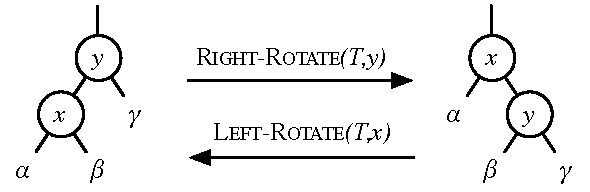
\includegraphics{rotation}
\par\end{center}

The pseudocode for \proc{Left-Rotate} assumes that $\attrib{x}{right} \neq \attrib{T}{nil}$

\begin{codebox}
\Procname{\proc{Left-Rotate}(T,x)}
\li $y \gets \attrib{x}{right}$   \>\>\>\>\>\Comment set $y$ (extract it from $x$)
\li $\attrib{x}{right} \gets \attrib{y}{left}$ \>\>\>\>\>\Comment save $y$'s left subtree into $x$'s right subtree
\li \If $\attrib{x}{right} \neq \attrib{T}{nil}$
\li   \Then $\attribb{y}{left}{p} \gets x$ \End
\li $\attrib{y}{p} \gets \attrib{x}{p}$    \>\>\>\>\>\Comment link $x$'s parent to $y$
\li \If $\attrib{x}{p} \isequal \attrib{T}{nil}$
\li   \Then $\attrib{T}{root} \gets y$  
\li \ElseIf $x \isequal \attribb{x}{p}{left}$
\li \> $\attribb{x}{p}{left} \gets y$
\li \Else $\attribb{x}{p}{right} \gets y$  \End
\li $\attrib{y}{left} \gets x$    \>\>\>\>\>\Comment put $x$ on $y$'s left
\li $\attrib{x}{p} \gets y$
\end{codebox}

Symmetrically the pseudocode for \proc{Right-Rotate} assumes that
$\attrib{y}{left} \neq \attrib{T}{nil}$. We can easily obtain it
from \proc{Left-Rotate} substituting $x$ with $y$ and $right$
with $left$.


\subsubsection{AVL Trees}

An \emph{AVL-tree} is a binary tree where the heights of the two child
subtrees of any node differ by at most one; therefore, it is also
said to be height-balanced.

The \emph{balance factor} of a node is the height of its left subtree
minus the height of its right subtree. A node with balance factor
1, 0, or \textminus{}1 is considered balanced while a node with any
other balance factor is considered unbalanced and requires rebalancing
the tree.


\paragraph{Insertion}

The pseudocode for \proc{AVL-Insert} assumes that every node $x$
in the AVL-tree stores its balance factor $bf$. Every leaf and newly
inserted node $z$ have $bf=0$.

\begin{codebox}
\Procname{$\proc{AVL-Insert}(T,z)$}
\li $\proc{TreeInsert}(T,z)$
\li \If $\attribb{z}{p}{left} \isequal z$   \>\>\>\>\>\>\>\> \Comment changes balance factor in $z$'s parent
\li    \Then $\attribb{z}{p}{bf} = \attribb{z}{p}{bf} + 1 $
\li \Else $\attribb{z}{p}{bf} = \attribb{z}{p}{bf} -1 $ \End
\li $x \gets \attrib{z}{p}$
\li \While $x \neq \const{nil}$ and $\attrib{x}{bf} \neq 0$ and $|\attrib{x}{bf}|<2$  
    \>\>\>\>\>\>\>\> \Comment propagates balance factor changes
    \Do
\li   \If $\attribb{x}{p}{left} \isequal x$
\li     \Then $\attribb{x}{p}{bf} = \attribb{x}{p}{bf} + 1 $
\li   \Else $\attribb{x}{p}{bf} = \attribb{x}{p}{bf} -1 $ \End
\li   $ x \gets \attrib{x}{p}$ 
    \End
\li \If $ \attrib{x}{bf} \isequal -2 $   \>\>\>\>\>\>\>\> \Comment $x$'s right subtree is unbalanced
\li   \Then \If $ \attribb{x}{right}{bf} \isequal -1 $
\li           \Then $\proc{Left-Rotate}(x)$
\li         \Else $\proc{Right-Rotate}(\attrib{x}{right})$
\li         $\proc{Left-Rotate}(x)$
            \End
    \End
\li \If $ \attrib{x}{bf} \isequal 2 $     \>\>\>\>\>\>\>\> \Comment $x$'s left subtree is unbalanced
\li   \Then \If $ \attribb{x}{left}{bf} \isequal 1 $
\li           \Then $\proc{Right-Rotate}(x)$
\li         \Else $\proc{Left-Rotate}(\attrib{x}{left})$
\li         $\proc{Right-Rotate}(x)$
            \End
    \End
\end{codebox}


\paragraph{Deletion}

The overall strategy for deleting a node $z$ from an AVL tree $T$
has the same three basic cases we have already seen in BSTs. 
\begin{itemize}
\item If $z$ has no children, then we simply remove it by modifying its
parent to replace $z$ with \const{nil} as its child.
\item If $z$ has just one child, then we elevate that child to take $z$'s
position in the tree by modifying $z$'s parent to replace $z$ by
$z$'s child.
\item If $z$ has two children, then we find $z$'s successor $y$ which
is contained in $z$'s right subtree (it is the smallest element greater
than $z$) and have $y$ take $z$'s position in the tree. The rest
of $z$'s original right subtree becomes $y$'s new right subtree,
and $z$'s left subtree becomes $y$'s new left subtree. After deletion,
retrace the path back up the tree from $y$'s parent to the root,
adjusting the balance factors as needed. The retracing can stop if
the balance factor becomes \textminus{}1 or +1 indicating that the
height of that subtree has remained unchanged. If the balance factor
becomes 0 then the height of the subtree has decreased by one and
the retracing needs to continue. If the balance factor becomes \textminus{}2
or +2 then the subtree is unbalanced and needs to be rotated to fix
it. If the rotation leaves the subtree's balance factor at 0 then
the retracing towards the root must continue since the height of this
subtree has decreased by one. This is in contrast to an insertion
where a rotation resulting in a balance factor of 0 indicated that
the subtree's height has remained unchanged.
\end{itemize}

\subsubsection{Red-Black trees}

A\emph{ red-black tree} is a binary tree that satisfies the following
red-black properties:
\begin{enumerate}
\item Every node is either red or black.
\item The root is black.
\item Every leaf (\const{nil}) is black. 
\item If a node is red, then both its children are black.
\item For each node $x$, all simple paths form $x$ to descendant leaves
contain the same number of black nodes. We call such a number the\emph{
back-height} of $x$, denoted $\func{bh}(x)$. The black-height of
a tree is the black-height of its root.
\end{enumerate}
Note how the leaves here are simply the sentinel value \attrib{T}{nil}
which is used to treat a \const{nil} child of a node $x$ as an ordinary
node whose parent is $x$.

A red black tree with $n$ internal nodes has height at most $2\log(n+1)$.


\subsection{Union-Find}

A \emph{disjoint-set data structure} (or \emph{Union-Find data structure})
maintains a collection $\mathcal{S}=\{S_{1},S_{2},\ldots,S_{k}\}$
of disjoint dynamic sets and, for each element $x\in S_{i},\,1\leq i\leq k$
supports the following operations:
\begin{itemize}
\item $\proc{Make-Set}(x)$ which creates a new set whose only member is
$x$. Since sets are disjoint, we require that $x$ not already be
in some other set.
\item $\proc{Union}(x,y)$ which unites the dynamic sets that contain $x$
and $y$, say $S_{x}$ and $S_{y}$, into a new set that is $S_{x}\cup S_{y}$.
\item $\proc{Find-Set}(x)$ which returns the dynamic set that contains
$x$.
\end{itemize}
Usually each set is referenced by a representative, that is an element
$x$ of such a set and we represent the overall number of elements
$x$ in the data structure with $n$. Also, we assume that the $n$
$\proc{Make-Set}$ operations are the first $n$ operations performed
when building a new disjoint-set data structure.

Union-Find data structures are used to represent the connected components
of an undirected graph and in particular in Kruskal's Algorithm to
find the Minimum Spanning Tree in an undirected graph.


\subsubsection{Implementation}

Two implementations are possible: 
\begin{description}
\item [{linked-lists:}] each set is represented by its own linked list.
With this implementation, both $\proc{Make-Set}$ and $\proc{Find-Set}$
are easy, and require $O(1)$ time. To carry out $\proc{Make-Set}(x)$,
we create a new linked-list whose only object is $x$. For $\proc{Find-Set}(x)$,
we just follow the pointer from $x$ back to its set object and return
it. However $\proc{Union}(x,y)$ procedure requires an average of
$\Theta(n)$ time per call because, after appending $y$ to $x$,
we must update the pointers of all elements in $y$'s list.
\item [{forest:}] each set is represented by a rooted tree. A$\proc{Make-Set}$
operation simply creates a tree with just one node. We perform a $\proc{Find-Set}$
operation by simply following parent pointers until we find the root
of the tree. A $\proc{Union}$ operation causes the root of one tree
to point to the root of the other. 
\end{description}
%
\begin{table}[H]
\begin{centering}
\begin{tabular}{|c|c|}
\hline 
Operation & Cost\tabularnewline
\hline
\hline 
Make-Set & $O(1)$\tabularnewline
\hline 
Union & $O(\alpha(n))$\tabularnewline
\hline 
Find-Set & $O(\alpha(n))$\tabularnewline
\hline
\end{tabular}
\par\end{centering}

\caption{Cost of operations}



\end{table}
Note that these values refer to the optimal forest implementation.

There is a nice theorem that states that a sequence of $m$ $\proc{Make-Set}$,
$\proc{Union}$, and $\proc{Find-Set}$ operations, $n$ of which
are $\proc{Make-Set}$ operations, can be performed on a disjoint-set
forest in worst-case time $O(m\alpha(n))$. Note that, since each
$\proc{Union}$ operation reduces the number of sets by one, the maximum
number of such operations is $n-1$. Also note that $m\geq n$ and
that we assume that the first $n$ $\proc{Make-Set}$ operations are
the first $n$ operations performed.


\section{Sorting, selecting, searching%
\footnote{Chapters 2, 6, 7, 8, 9%
}}


\subsection{Insertion sort}

The \emph{insertion sort} algorithm is the most intuitive, yet inefficient,
sorting algorithm. It orders the sequence by inserting each element
in the right place in the sorted portion of the sequence.


\subsubsection{Implementation}

The following procedure takes as a parameter an array $A[1\twodots n]$
containing a sequence of numbers of length $n$ and sorts it \emph{in
place} by rearranging the numbers within the array itself. This means
the input array $A$ contains the sorted output sequence when the
procedure is finished.

\begin{codebox} 
\Procname{$\proc{Insertion-Sort}(A)$} 
\li \For $j \gets 2$ \To $\attrib{A}{length}$ 
      \Do 
\li   $\id{key} \gets A[j]$ 
\li   \Comment Insert $A[j]$ into the sorted sequence $A[1 \twodots j-1]$. 
\li   $i \gets j-1$ 
\li   \While $i > 0$ and $A[i] > \id{key}$ 
        \Do 
\li     $A[i+1] \gets A[i]$ 
\li     $i \gets i-1$ 
      \End 
\li   $A[i+1] \gets \id{key}$ 
     \End
\end{codebox}


\subsubsection{Time complexity}

$O(n^{2})$: When the array is reverse sorted order, which is the
worst case, we need to compare each element $A[j]$ with each element
in the entire sorted subarray $A[1\twodots j-1]$.


\subsection{Merge sort}

The \emph{merge sort }algorithm closely follows the Divide-and-Conquer
paradigm. Intuitively, it operates as follows:
\begin{description}
\item [{Divide:}] Divide the $n$-element sequence to be sorted into two
subsequences of $n/2$ elements each.
\item [{Conquer:}] Sort the two subsequences recursively using merge sort.
\item [{Combine:}] Merge the two sorted subsequences to produce the sorted
answer.
\end{description}
Merge sort does not sort in place but it is possible to devise a modified
version that does so.


\subsubsection{Implementation}

The following procedure assumes that the subarrays $A[p\twodots q]$
and $A[q+1\twodots r]$ are already sorted and it merges them to form
a single sorted subarray that replaces the current subarray $A[p\twodots r]$.

\begin{codebox}
\Procname{$\proc{Merge}(A,p,q,r)$}
\li $n_1 \gets q-p +1$
\li $n_2 \gets r-q $
\li let $L[1\twodots n_1+1]$ and $R[1\twodots n_2+1]$ be new arrays
\li \For $i \gets 1 \To n_1$
\li   \Do $L[i] \gets A[p+i-1]$ \End
\li \For $j \gets 1 \To n_2$
\li   \Do $R[j] \gets A[q+j]$ \End
\li $L[n_1+1] \gets \infty$
\li $R[n_2+1] \gets \infty$
\li $i \gets 1$
\li $j \gets 1$
\li \For $k \gets p \To r$
      \Do
\li   \If $L[i]\leq R[j]$
        \Then
\li     $A[k] \gets L[i]$
\li     $i \gets i+1$
\li   \Else $A[k] \gets R[j]$
\li     $j \gets j+1$
      \End
    \End
\end{codebox}

We can use the $\proc{Merge}$ procedure as a subroutine in the merge
sort algorithm. The following procedure sorts the elements in the
subarray $A[p\twodots r]$.

\begin{codebox}
\Procname{$\proc{Merge-Sort}(A,p,r)$}
\li \If $p<r$
      \Then
\li   $q \gets \lfloor (p+r)/2 \rfloor$
\li   $\proc{Merge-Sort}(A,p,q)$
\li   $\proc{Merge-Sort}(A,q+1,r)$
\li   $\proc{Merge}(A,p,q,r)$
      \End
\end{codebox}

To sort the entire array $A$ we make the initial call $\proc{Merge-Sort}(A,1,\attrib{A}{length})$.


\subsubsection{Time complexity}

$\Theta(n\log n)$, since the \proc{Merge} procedure, which runs
in $\Theta(n)$, is executed $\log n$ times.


\subsection{Heap sort}

The \emph{heap sort} algorithm works by exploiting the max-heap property
that the biggest element is always at the root. It swaps the root
of the heap with the last element in the array and then reorganizes
all the elements but the last one so that the data structure satisfies
again the max-heap property.


\subsubsection{Implementation}

The following procedure takes as a parameter an array $A[1\twodots n]$
and sorts it \emph{in place}. The procedure $\proc{Build-Max-Heap}(A)$
is not described in this document.

\begin{codebox}
\Procname{$\proc{Heap-Sort}(A)$}
\li $\proc{Build-Max-Heap}(A)$
\li \For $i \gets \attrib{A}{length} \Downto 2$
       \Do
\li    exchange $A[1]$ with $A[i]$
\li    $\attrib{A}{heap-size} \gets \attrib{A}{heap-size} - 1$
\li    $\proc{Max-Heapify}(A,1)$
\end{codebox}


\subsubsection{Time complexity}

$\Theta(n\log n)$, since the call to $\proc{Build-Max-Heap}$ takes
time $O(n)$ and each of the $n-1$ calls to $\proc{Max-Heapify}$
takes time $O(\log n)$.


\subsection{Quick sort}

The \emph{quick sort} algorithm is another example of application
of the Divide-and-Conquer paradigm. However, differently from merge
sort, it sorts\emph{ in place}. The three steps to sort a subarray
$A[p\twodots r]$ are:
\begin{description}
\item [{Divide:}] Partition (rearrange) the array$A[p\twodots r]$ into
(possibly empty) subarrays $A[p\twodots q-1]$ and $A[q+1\twodots r]$
such that each element of $A[p\twodots q-1]$ is less or equal to
$A[q]$, which is, in turn, less than or equal to each element of
$A[q+1\twodots r]$. Compute the index $q$ as part of this partition
procedure.
\item [{Conquer:}] Sort the two subarrays $A[p\twodots q-1]$ and $A[q+1\twodots r]$
by recursive calls to quick sort.
\item [{Combine:}] Because the subarrays are already sorted, no work is
needed to combine them: the entire array $A[p\twodots r]$ is now
sorted.
\end{description}

\subsubsection{Implementation}

The following procedure implements quick sort.

\begin{codebox}
\Procname{$\proc{Quick-Sort}(A,p,r)$}
\li \If $p<r$ \Then 
\li   $q \gets \proc{Partition}(A,p,r)$
\li   $\proc{Quick-Sort}(A,p,q-1)$
\li   $\proc{Quick-Sort}(A,q+1,r)$
    \End
\end{codebox}

The key to the algorithm is the $\proc{Partition}$ procedure, which
rearranges the subarray $A[p\twodots r]$ in place by partitioning
the array in three (possibly empty) regions: elements $\leq x$, elements
$>x$ and $x$.

\begin{codebox}
\Procname{$\proc{Partition}(A,p,r)$}
\li $x \gets A[r]$   \>\>\>\>\>\>\>  \Comment selects the $pivot$
\li $i \gets p-1$  
\li \For $j \gets p \To r-1$    \>\>\>\>\>\>\>  \Comment separates the elements $\leq x$ from the ones $>x$
       \Do
\li    \If $A[j] \leq x$
          \Then
\li       $i \gets i+1$
\li       exchange $A[i]$ with $A[j]$
       \End
    \End
\li exchange $A[i+1]$ with $A[r]$  \>\>\>\>\>\>\>  \Comment moves the pivot "in the middle"
\li \Return  $i+1$
\end{codebox}

To sort the entire array $A$ we make the initial call $\proc{Quick-Sort}(A,1,\attrib{A}{length})$.


\subsubsection{Time complexity}

The running time of quick sort depends on whether the partition is
balanced ($\Theta(n\log n)$) or unbalanced ($\Theta(n^{2})$). The
average-case running time of quick sort is $O(n\log n)$ which is
much closer to the best case than to the worst case.

It is possible to devise a randomized version of quick sort where
the pivot is chosen randomly among the elements of the subarray $A[p\twodots r]$
yielding an average running time of $O(n\log n)$.


\subsection{Lower bounds for sorting}

All the previous sorting algorithms belong to the family of the so
called \emph{comparison sorts}. This family is important because we
can prove that any comparison sort algorithm requires $\Omega(n\log n)$
comparisons in the worst case. 

This means that heap sort and merge sort are \emph{asymptotically
optimal} comparison sorts.


\subsection{Quick select}

A \emph{selection algorithm} is an algorithm for finding the $i$th
smallest number in a set of $n$ (distinct) elements. Such a number
is called the $i$th order statistic of the set. This includes the
cases of finding the minimum (first order statistics), maximum ($n$th
order statistics), and median ($\lfloor(n+1)/2\rfloor$ lower median
or $\lceil(n+1)/2\rceil$ upper median) elements.

We can solve the selection problem in $O(n\log n)$ time, since we
can sort the numbers and then simply access the $i$th element in
the output array. However, there are $\Theta(n)$ time algorithms
to determine the minimum and the maximum and the following algorithm,
to solve the general selection problem, is faster.


\subsubsection{Implementation}

The following procedure implements the quick select algorithm which
works similarly to quick sort: it takes as input the array $A[p\twodots r]$
and returns its $i$th smallest element.

\begin{codebox}
\Procname{$\proc{Randomized-Select}(A,p,r,i)$}
\li \If $p \isequal r$ 
\li   \Then \Return $A[p]$
    \End
\li $q \gets \proc{Randomized-Partition}(A,p,r)$
\li $k \gets q-p+1 $
\li \If $i \isequal k $     \>\>\>\>\>\>\>\>\> \Comment the pivot is the answer
\li   \Then \Return $A[q]$  
\li \ElseIf $i<k$  
\li   \Return $\proc{Randomized-Select}(A,p,q-1,i)$  \>\>\>\>\>\>\>\>\>  \Comment continue search within the smaller elements
\li \Else \Return $\proc{Randomized-Select}(A,q+1,r,i)$  \>\>\>\>\>\>\>\> \Comment continue search within the bigger elements
    \End
\end{codebox}

The algorithm uses the $\proc{Randomized-Partition}$ procedure, which
is the randomized version of the $\proc{Partition}$ procedure used
by quick sort.

\begin{codebox}
\Procname{$\proc{Randomized-Partition}(A,p,r)$}
\li $i \gets \proc{Random}(p,r)$
\li exchange $A[r]$ with $A[i]$
\li \Return  $\proc{Partition}(A,p,r)$
\end{codebox}


\subsubsection{Time complexity}

The expected running time of $\proc{Randomized-Select}$ is $\Theta(n)$.
This is due to the fact that, as in quick sort, we partition the input
array recursively but unlike quick sort, which recursively processes
both sides of the partition, $\proc{Randomized-Select}$ works only
on one side of the partition. (the one containing the i-th element)


\subsection{Binary search}

See page \pageref{bin-search}.


\section{Patterns in algorithms design%
\footnote{Chapters 15, 16%
}}


\subsection{Dynamic Programming}

An \emph{optimization problem} needs to have the following two characteristics
in order for DP to apply: 
\begin{itemize}
\item expose \emph{optimal substructure}, which means that an optimal solution
to a problem contains optimal solutions to smaller subproblems (exactly
like in Divide-and-Conquer)
\item have \emph{overlapping problems}, which means that a subproblem is
revisited multiple times. If problems are not overlapping it doesn't
make sense to store the partial results and a Divide-and-Conquer algorithm
is probably a better choice.
\end{itemize}
DP algorithms work in a bottom-up fashion by finding optimal solutions
to subproblems (often all of them) and then making a choice among
these subproblems to select which one will be used in solving the
bigger subproblems and ultimately the original problem.


\subsubsection{Longest Common Subsequence (LCS)}

Given a sequence $X=\langle x_{1},x_{2},\ldots,x_{m}\rangle$, another
sequence $Z=\langle z_{1},z_{2},\ldots,z_{k}\rangle$ is a subsequence
of $X$ if there exists a strictlyr increasing sequence $\langle i_{1},i_{2},\ldots,i_{k}\rangle$
of indices of $X$ such that for all $j=1,2,\ldots,k$, we have $x_{i_{j}}=z_{j}$.
Given two sequences $X$ and $Y$, we say that a sequence $Z$ is
a common subsequence of $X$ and $Y$ if $Z$ is a subsequence of
both $X$ and $Y$.

In the longest subsequence problem, we are given two sequences $X=\langle x_{1},x_{2},\ldots,x_{m}\rangle$
and $Y=\langle y_{1},y_{2},\ldots,y_{n}\rangle$ and wish to find
a maximum length common subsequence $Z=\langle z_{1},z_{2},\ldots,z_{k}\rangle$
of $X$ and $Y$.


\paragraph{Optimal substructure and overlapping problems}

In order to apply DP we need to show that the problem has optimal
substructure. This step will also offer a hint on how to use the subproblems
solution to find the solution to the problem. 

Let $X=\langle x_{1},x_{2},\ldots,x_{m}\rangle$ and $Y=\langle y_{1},y_{2},\ldots,y_{n}\rangle$
be sequences, and let $Z=\langle z_{1},z_{2},\ldots,z_{k}\rangle$
be any LCS of $X$ and $Y$.
\begin{enumerate}
\item If $x_{m}=y_{n}$, then $z_{k}=x_{m}=y_{n}$ and $Z_{k-1}$ is an
LCS of $X_{m-1}$ and $Y_{n-1}$.
\item If $x_{m}\neq y_{n}$, then $z_{k}\neq x_{m}$ implies that $Z$ is
an LCS of $X_{m-1}$ and $Y$.
\item If $x_{m}\neq y_{n}$, then $z_{k}\neq y_{n}$ implies that $Z$ is
an LCS of $X$ and $Y_{n-1}$.
\end{enumerate}
We can also see how to find an LCS of $X$ and $Y$, we may need to
find the LCS of $X$ and $Y_{n-1}$ and of $X_{m-1}$ and $Y$. 


\paragraph{Implementation}

We can define $c[i,j]$ to be the length of an LCS of the sequences
$X_{i}$ and $Y_{j}$. The optimal substructure of the LCS problem
gives the recursive formula \[
c[i,j]=\begin{cases}
0 & \text{if \ensuremath{i=0}or \ensuremath{j=0}}\\
c[i-1,j-1]+1 & \text{if \ensuremath{i,j>0}and \ensuremath{z_{i}=y_{j}}}\\
max(c[i,j-1],c[i-1,j]) & \text{if \ensuremath{i,j>0}and \ensuremath{z_{i}\neq y_{j}}}\end{cases}\]


We can use such a recursion to write an algorithm that takes in input
$X$ and $Y$ and stores the values of $c[i,j]$ in a table $c[0\twodots m,0\twodots n]$,
and it computes the entries in row-major order. The procedure also
maintains a table $b[1\twodots m,1\twodots n]$ to help us construct
an optimal solution: intuitively, $b[i,j]$ points to the table entry
corresponding to the optimal subproblem solution chosen when computing
$c[i,j]$. The procedure returns tables $b$ and $c$ and the LCS
for $X$ and $Y$ is stored in $c[m,n]$.

\begin{codebox}
\Procname{\proc{LCS-Length}($X$,$Y$)}
\li $m \gets \attrib{X}{length}$
\li $n \gets \attrib{Y}{length}$
\li let $c[0\twodots m,0\twodots n]$ and $b[1\twodots m,1\twodots n]$ be new tables
\li \For $i \gets 1 \To m $ \Do
\li   $c[i,0] \gets 0$ \End
\li \For $j \gets 0 \To n $ \Do
\li   $c[0,j] \gets 0$ \End
\li \For $i \gets 1 \To m $ \Do
\li    \For $j \gets 1 \To n $ \Do
\li      \If $x_i \isequal y_j$ \Then
\li          $c[i,j] \gets c[i-1,j-1] + 1$
\li          $b[i,j] \gets "\nwarrow"$
\li      \ElseIf $c[i-1,j] \geq c[i,j-1] $ \Then
\li          $c[i,j] \gets c[i-1,j] $
\li          $b[i,j] \gets "\uparrow"$
\li      \Else $c[i,j] \gets c[i,j-1] + 1$
\li          $b[i,j] \gets "\leftarrow"$
         \End \End \End
\li \Return $c$ and $b$
\end{codebox}

We can then print the LCS using table $b$ and the following procedure.
The initial call is \proc{Print-LCS}($b$,$X$,\attrib{X}{length},\attrib{Y}{length}).

\begin{codebox}
\Procname{\proc{Print-LCS}($b$,$X$,$i$,$j$)}
\li \If $i \isequal 0$ or $j \isequal 0$ \Then
\li    \Return \End
\li \If $b[i,j] \isequal "\nwarrow"$ \Then 
\li    \proc{Print-LCS}($b$,$X$,$i-1$,$j-1$)
\li    print $x_i$ 
\li \ElseIf $b[i,j] \isequal "\uparrow"$ \Then 
\li    \proc{Print-LCS}($b$,$X$,$i-1$,$j$)
\li \Else \proc{Print-LCS}($b$,$X$,$i$,$j-1$)
\end{codebox}


\subsubsection{Other problems that are solvable with DP algorithms}


\paragraph{Rod cutting problem }

Given a rod of length $n$ and a table of prices $p_{i}$ for $i=1,2\ldots,n$,
determine the maximum revenue $r_{n}$ obtainable by cutting up the
rod and selling the pieces. Note that if the price $p_{n}$ for a
rod of length $n$ is large enough, an optimal solution may require
no cutting at all.

The following dynamic programming algorithm takes as input an array
$p[1\twodots n]$ of prices and an integer $n$ and returns an array
$r[0\twodots n]$ in which it saves the results of the subproblems
and an array $s[0\twodots n]$ containing the optimal size of the
first piece to cut off when solving a subproblem of size $j$.

\begin{codebox}
\Procname{\proc{Cut-Rod}($p,n$)}
\li let $r[0\twodots n]$ and $s[0\twodots n]$ be new arrays
\li $r[0] \gets 0$
\li \For $j \gets 1 \To n$ \Do
\li   $q \gets -\infty$
\li   \For $i \gets 1 \To j$ \Do
\li     \If $q<p[i]+r[j-i]$ \Then
\li        $q \gets p[i]+r[j-i]$
\li        $s[j] \gets i$ \End  \End
\li   $r[j] \gets q$ \End
\li \Return $r$ and $s$
\end{codebox}


\paragraph{0-1 knapsack problem}

We are given $n$ items. Each item $i$ has a value of $v_{i}$ dollars
and a weight $w_{i}$ pounds which are nonnegative integers. Given
a bag whose capacity is $W$ what is the maximum value that we can
carry knowing that we can either carry an item (therefore $1\cdot w_{i}$)
or leave it behind (therefore $0\cdot w_{i}$) but not carry a portion
of it?

If $i$ is the highest-numbered item in an optimal solution $S$ for
$W$ pounds and items $1\twodots n$. Then $S\lyxmathsym{\textasciiacute}=S\lyxmathsym{\textminus}\{i\}$
must be an optimal solution for $W-w_{i}$ pounds and items $1\twodots i$-1
pounds, and the value of the solution $S$ is $v_{i}$ plus the value
of the subproblem solution $S\lyxmathsym{\textasciiacute}$. Assuming
$c[i,w]$ to be the value of the solution for items $1\twodots1$
and maximum weight $w$ we can formalize the previous statement as\[
c[i,w]=\begin{cases}
0 & \text{if }i=0\text{ or }w=0\\
c[i-1,w] & \text{if }w_{i}>w\\
\max(v_{i}+c[i-1,w-w_{i}],c[i-1,w]) & \text{if }i>1\text{ and }w\geq w_{i}\end{cases}\]


The following dynamic programming algorithm takes as input the arrays
of values $v[1\twodots n]$ and weights $w[1\twodots n]$, the capacity
$W$ and returns a table $c[0\twodots n,0\twodots W]$ which contains
the values of the solutions for all subproblems. At the end of the
computation $c[n,W]$ contains the maximum value we can carry.

\begin{codebox}
\Procname{\proc{0-1-Knapsack}($v,w,W$)}
\li $n \gets \attrib{v}{length}$
\li let $c[0\twodots n,0\twodots W]$ be a new table
\li \For $w \gets 0 \To W$ \Do
\li   $c[0,w] \gets 0$ \End
\li \For $i \gets 1 \To n$ \Do
\li   $c[i,0] \gets 0$ \End

\li \For $i \gets 1 \To n$ \Do
\li    \For $w \gets 1 \To W$ \Do
\li       \If $w[i] \leq w $ \Then
\li          \If $v[i] + c[i-1,w-w[i]]> c[i-1,w]$ \Then
\li               $c[i,w] \gets v[i] + c[i-1,w-w[i]]$
\li          \Else $c[i,w] \gets c[i-1,w]$ \End
\li       \Else $c[i,w] \gets c[i-1,w] $ \End \End \End
\li \Return $c$
\end{codebox}

To find out which items are included in the solution we need to start
at c$[n,W]$ and tracing where the optimal values came from. If $c[i,w]=c[i\lyxmathsym{\textminus}1,w]$,
then item $i$ is not part of the solution, and we continue tracing
with $c[i\lyxmathsym{\textminus}1,w]$. Otherwise item $i$ is part
of the solution, and we continue tracing with $c[i\lyxmathsym{\textminus}1,w\lyxmathsym{\textminus}w[i]]$.


\subsection{Greedy Algorithms}

A greedy algorithm obtains an optimal solution to a problem by making
a sequence of choices that looks best at the moment (i.e. a local
optimal choice) hoping that it will lead to a globally optimal solution. 

An optimization problem needs to have the following two characteristics
in order to be efficiently solvable with a greedy algorithm: 
\begin{itemize}
\item expose \emph{optimal substructure}, exactly as DP
\item have a \emph{greedy-choice property}, which means that we can assemble
a globally optimal solution by making a locally optimal (greedy) choices. 
\end{itemize}
In DP algorithms we make a choice at each step, but the choice usually
depends on the solutions to subproblems. In greedy algorithms, we
make whatever choice seems best at the moment and then solve the subproblem
that remains. 

A DP algorithm proceeds bottom-up, whereas a greedy strategy usually
progresses in a top-down fashion, making one greedy choice after another,
reducing each given problem instance to a smaller one.


\subsubsection{Proving correctness and optimality }

How can we prove that the solution found by a greedy algorithm is
optimal if we don't even know what the optimal solution is? Of course
if we can prove that an optimal solution exists and is the same one
found by the greedy algorithm then we are done. There are cases where
this is not possible and therefore we need to use techniques that
only use a property of the optimal solution which can in turn be used
to prove the correctness and optimality of a greedy algorithm.
\begin{itemize}
\item Greedy algorithm stays ahead. Show that after each step of the algorithm,
the solution it finds is at least as good as any other algorithm's
solution. 
\item Exchange argument. Gradually transform any solution to the one found
by the greedy algorithm without hurting its quality.
\item Structural. Discover a simple \textquotedbl{}structural\textquotedbl{}
bound asserting that every possible solution must have a certain value.
Then show that your algorithm always achieves this bound.
\end{itemize}

\subsubsection{Huffman codes}

Huffman's greedy algorithm builds a variable length binary character
code, in which each character is represented by a unique binary string,
which we call codeword. The goal is to give more frequent character
short codewords and infrequent characters long codewords to achieve
data compression.

In the pseudocode that follows , we assume $C$ is a set of $n$ characters
and that each character $c\in C$ is an object with an attribute \attrib{c}{freq}
giving its frequency. The algorithm builds a tree $T$ corresponding
to the optimal code in a bottom-up fashion and uses a min-priority
queue $Q$, keyed on the $freq$ attribute, to identify the two least-frequent
objects to merge together. 

\begin{codebox}
\Procname{$\proc{Huffman}(C)$}
\li $n \gets |C|$
\li $Q \gets C$
\li \For $i \gets 1 \To n-1$ \Do
\li   allocate a new node $z$
\li   $\attrib{z}{left} \gets x \gets \proc{Extract-Min}(Q)$
\li   $\attrib{z}{right} \gets y \gets \proc{Extract-Min}(Q)$
\li   $\attrib{z}{freq} \gets \attrib{x}{freq} + \attrib{y}{freq}$
\li   $\proc{Insert}(Q,z)$
    \End
\li \Return \proc{Extract-Min}(Q) \>\>\>\>\>\>  \Comment returns the root of the tree
\end{codebox}

Running time of this algorithm is $O(n\log n)$ since priority queue
operations run in $\log n$ time and the main loop executes $n-1$
times.


\subsubsection{Other problems that are solvable with greedy algorithms}


\paragraph{Activity selection problem }

In this problem we are given a set of activities $A=\{a_{1},\ldots,a_{n}\}$
and their start and finish times $s_{i}$ and $f_{i}$ and we need
to find the maximum subset of mutually compatible activities. Two
activities $i$ and $j$ are compatible if they don't overlap. 

To solve this problem we consider activities in increasing order of
finish time and we schedule them provided they are compatible with
the ones already taken. Here $S$ is the set of selected activities.

\begin{codebox}
\Procname{\proc{Activity-selection}($A$)}
\li \proc{Sort}($A$)  \>\>\>  \Comment in increasing order of finish time $f_i$
\li $S \gets \emptyset$
\li \For $i \gets 1 \To n$ \Do
\li   \If $a_i$ is compatible with $S$ \Then
\li     $S \gets S \cup a_i$ \End \End
\li \Return $S$
\end{codebox}


\paragraph{Activity partitioning problem}

In this problem we are given a set of activities $A=\{a_{1},\ldots,a_{n}\}$
and their start and finish times $s_{i}$ and $f_{i}$ and we need
to find the minimum number of {}``slots'' necessary to schedule
all activities. Clearly two activities can't overlap in the same slot. 

To solve this problem we consider activities in increasing order of
start time. Here $s$ is the number of a slots.

\begin{codebox}
\Procname{\proc{Activity-partitioning}($A$)}
\li \proc{Sort}($A$)  \>\>\>  \Comment in increasing order of start time $s_i$
\li $s \gets 0$
\li \For $i \gets 1 \To n$ \Do
\li   \If $a_i$ is compatible with some slot $k$ \Then
\li     schedule $a_i$ in slot $k$ 
\li   \Else allocate a new slot $s+1$
\li   schedule $a_i$ in slot $s+1$
\li   $s \gets s + 1$ \End \End
\li \Return $s$
\end{codebox}


\paragraph{Lateness minimization problem }

In this problem we are given a set of activities $A=\{a_{1},\ldots,a_{n}\}$,
their start and finish times $s_{i}$ and $f_{i}$ and their due time
(deadline) $d_{i}$. We can also define, for each job $i$, lateness
as $l_{i}=\max(0,f_{i}-d_{i})$ and the amount of time required to
complete as $t_{i}=f_{i}-s_{i}$. $ $

Our goal is to schedule all activities minimizing maximum lateness
$L=\underset{i\in\{[1\twodots n]\}}{\max l_{i}}$

To solve this problem we consider activities in increasing order of
deadline (earlies deadline activities come first). At the end of the
algorithm $A$ contains the scheduled activities.

\begin{codebox}
\Procname{\proc{Lateness-Minimization}($A$)}
\li \proc{Sort}($A$)  \>\>\>  \Comment in increasing order of deadline $d_i$
\li $t \gets 0$
\li \For $i \gets 1 \To n$ \Do
\li   schedule $a_i$ in interval $[t,t+t_i]$ 
\li   $s_i \gets t$
\li   $f_i \gets t+t_i$
\li   $t \gets t + t_i$  \End
\end{codebox}


\paragraph{Optimal off-line caching problem}

In this problem we are given a cache with capacity $k$ and a sequence
of requests $d_{1},d_{2},\ldots,d_{m}$. We want to find an eviction
schedule (i.e. decide which element in the cache we want to overwrite)
that minimizes the number of cache misses.

The optimal solution is to evict the item that is not requested until
\emph{farthest in the future}. 


\paragraph{Coin changing problem}

In this problem we are given the currency denominations $D=\{1,5,10,25,100\}$
(US coinage) and and a certain amount $x$. We need to devise a method
to pay the amount $x$ using the fewest number of coins.

The problem can be solved using the so called cashier's algorithm,
which at each iteration adds the coin of largest value that does not
take us past the amount to be paid.

\begin{codebox}
\Procname{\proc{Coin-Change}($D$)}
\li \proc{Sort}($D$)  \>\>\>  \Comment in increasing order
\li $S \gets \emptyset$
\li \While $x \neq 0$ \Do
\li   let $k$ be the largest integer such that $c_k < x$
\li   \If $k \isequal 0$ \Then
\li      \Return \Error \End
\li   $x \gets x - c_k$
\li   $S \gets S \cup \{ k \}$  \End
\li \Return $S$
\end{codebox}

Note that the previous algorithm is optimal for US coinage. If we
use different denomiations we might need a different algorithm that
uses Dynamic Programming.


\paragraph{Fractional knapsack problem }

In this problem we are given a set of items $A=\{a_{1},\ldots,a_{n}\}$,
each with a weight $w_{i}$ and a value $v_{i}$ and a container of
capacity $x$. We need to find the set of items (or fraction of items)
so that the total weight is less than $x$ and the total value is
as large as possible.

The problem can be solved by sorting the items in decreasing order
of revenue $r_{i}=\frac{v_{i}}{w_{i}}$ and then filling the container
up to $x$ by taking a fraction of the last item if such an item doesn't
fit entirely.


\section{Graphs%
\footnote{Chapters 22, 23, 24, 25%
}}


\subsection{Data structures}


\subsubsection{Adjacency-list}

The \emph{adjacency-list} \emph{representation} of a graph $G=(V,E)$
consists of an array $Adj$ of $n$ linked lists, one for each vertex
$u\in V$, such that $Adj[u]$ contains all the vertices adjacent
to $u$ in $G$.
\begin{itemize}
\item If $G$ is directed then the sum of the lengths of all the adjacency
lists is $m$.
\item If $G$ is undirected then the sum of the lengths of all the adjacency
lists is $2m$.
\item The amount of memory required to store the adjacency-list representation
of $G$ is $\Theta(n+m)$: this is the major advantage of this representation.
\item The amount of time needed to scan the entire data structure is $\Theta(n+m)$:
this is an advantage of this representation.
\item The amount of time to search for $v$ in the adjacency-list $Adj[u]$
is $O(\deg(u))$ because in the worst case we need to scan $G.Adj[u]$
entirely. 
\item The amount of time to check if a given edge $(u,v)$ is present in
the graph is $O(\deg(u))$ that is the same time needed to search
for $v$ in $Adj[u]$: this is the major drawback of this representation.
\item Generally speaking this representation is better for sparse and/or
big graphs.
\end{itemize}

\subsubsection{Adjacency-matrix}

The \emph{adjacency-matrix} \emph{representation} of a graph $G=(V,E)$
consists of a matrix $A=(a_{ij})$ such that \[
a_{ij}=\begin{cases}
1 & \text{if }(i,j)\in E\\
0 & \text{otherwise}\end{cases}\]

\begin{itemize}
\item If $G$ is undirected then $A=A^{T}$, that is $A$ is symmetrical.
\item The amount of memory required to store the adjacency-matrix representation
is $\Theta(n^{2})$, independently from the number of edges: this
is the major drawback of this representation
\item The amount of time needed to scan the entire data structure is $\Theta(n^{2})$
that is asymptotically more complex than the time needed to scan the
adjacency-list: this is a drawback of this representation.
\item The amount of time to check if a given edge $(u,v)$ is present in
the graph is $\Theta(1)$ because we just need to check the relative
entry in the adjacency-matrix: this is the major advantage of this
representation.
\item Generally speaking this representation is better for dense and/or
small graphs.
\end{itemize}

\subsection{Elementary Algorithms}


\subsubsection{Breadth-first search (BFS)}

Given a graph $G=(V,E)$ and a distinguished source vertex $s$ this
algorithm:
\begin{itemize}
\item assumes an adjacency-list representation;
\item works both on directed and undirected graphs;
\item systematically explores the edges of $G$ to {}``discover'' every
vertex that is reachable from $s$ (can be used to identify the connected
components if executed on multiple sources);
\item computes the shortest-path%
\footnote{We define the \emph{shortest-path distance} $\delta(s,v)$ from $s$
to $v$ as the minimum number of edges in any path from vertex $s$
to vertex $v$; if there is no path from $s$ to $v$ then $\delta(s,v)=\infty$.

We call a simple path of length $\delta(s,v)$ from $s$ to $v$ a
\emph{shortest path} from $s$ to $v$. 

Note that this is a particular case of the more general shortest-path
problem which involves edges with different weights.%
} from $s$ to every reachable vertex $v$;
\item produces a \emph{breadth-first tree} with root $s$ that contains
all reachable vertices (which can be used to print the (reverse-)shortest-path
from $s$ to any vertex $v$);
\item uses a \emph{queue} to store the neighbors (which ensures that the
algorithm discovers all the vertices at distance $k$ from $s$ before
discovering vertices at distance $k+1$;
\item has a running time of $O(n+m)$, that is a time linear in the size
of the adjacency-list representation (because each vertex is enqueued/dequeued
only once and the adjacency-list of each vertex is scanned only when
the vertex is dequeued.
\end{itemize}
\begin{codebox}
\Procname{$\proc{BFS}(G,s)$}
\li \For each vertex $u \in \attrib{G}{V}-\{s\}$
      \Do   \>\>\>\>\>\> \Comment initialize vertices
\li   $\attrib{u}{color} \gets \const{white}$
\li   $\attrib{u}{d} \gets \infty $
\li   $\attrib{u}{\pi} \gets \const{nil}$
    \End
\li $\attrib{s}{color} \gets \const{gray}$  \>\>\>\>\>\>\> \Comment inintializes $Q$ with $s$
\li $\attrib{s}{d} \gets 0$
\li $\attrib{s}{\pi} \gets \const{nil}$
\li $Q \gets \emptyset$
\li $\proc{Enqueue}(Q,s)$
\li \While $Q \neq \emptyset$
      \Do 
\li   $u \gets \proc{Dequeue}(Q)$    \>\>\>\>\>\> \Comment fetch next vertex to be visited
\li   \For each $v\in \attrib{G}{Adj[u]}$  \>\>\>\>\>\> \Comment add neighbors to queue
        \Do
\li     \If $\attrib{u}{color} \isequal \const{white}$
          \Then
\li       $\attrib{v}{color} \gets \const{gray}$
\li       $\attrib{v}{d} \gets \attrib{u}{d} +1$
\li       $\attrib{v}{\pi} \gets u$
\li       $\proc{Enqueue}(Q,v)$
        \End
      \End
\li    $\attrib{u}{color} \gets \const{black}$  \>\>\>\>\>\> \Comment mark as visited
    \End
\end{codebox}


\subsubsection{Depth-first search (DFS)}

Given a graph $G=(V,E)$ this algorithm:
\begin{itemize}
\item assumes an adjacency-list representation;
\item works both on directed and undirected graphs;
\item systematically explores the edges out of the most recently discovered
vertex $v$ that still has unexplored edges leaving it and, once all
of $v$'s edges have been explored, the search {}``backtracks''
to explore edges leaving the vertex from which $v$ was discovered;
\item produces a \emph{depth-first forest} $G_{\pi}$comprising several
\emph{depth-first trees};
\item it's recursive, which means it implicitly uses a \emph{stack} to store
the vertices that have been \emph{discovered} but not yet \emph{finished};
\item has a running time of $O(n+m)$, that is a time linear in the size
of the adjacency-list representation (because the {}``visit procedure''
is called once for every vertex and has a running time of $\sum_{v\in V}|Adj[v]|=\Theta(m)$.
\end{itemize}
\begin{codebox}
\Procname{$\proc{DFS}(G)$}
\li \For each vertex $u \in \attrib{G}{V}$
      \Do   \>\>\>\>\> \Comment initialize vertices
\li   $\attrib{u}{color} \gets \const{white}$
\li   $\attrib{u}{\pi} \gets \const{nil}$
    \End
\li $time \gets 0$
\li \For each $u\in \attrib{G}{V}$  \>\>\>\>\>\> \Comment make sure we visit all nodes
        \Do
\li     \If $\attrib{u}{color} \isequal \const{white}$
          \Then
\li       $\proc{DFS-Visit}(G,u)$
        \End
      \End
    \End
\end{codebox}

\begin{codebox}
\Procname{$\proc{DFS-Visit}(G,u)$}
\li $time \gets time +1$
\li $\attrib{u}{d} \gets time$   \>\>\>\>\>\> \Comment set $discovery$ time
\li $\attrib{u}{color} \gets \const{gray}$
\li \For each $v\in \attrib{G}{Adj[u]}$  \>\>\>\>\>\> \Comment add neighbors to stack
      \Do
\li   \If $\attrib{v}{color} \isequal \const{white}$
          \Then
\li       $\attrib{v}{\pi} \gets u$
\li       $\proc{DFS-Visit}(G,v)$
      \End
    \End
\li $\attrib{u}{color} \gets \const{black}$  \>\>\>\>\>\> \Comment mark as visited
\li $time \gets time +1$
\li $\attrib{u}{f} \gets time$  \>\>\>\>\>\> \Comment set $finishing$ time
\end{codebox}


\paragraph{Edge classification}

DFS can be used to classify the edges of the input graph $G$. We
can define four edges types in terms of the depth-first forest $G_{\pi}$:
\begin{itemize}
\item \emph{Tree edges} are edges in $G_{\pi}$. Edge $(u,v)$ is a tree
edge if $v$ was first discovered by exploring edge $(u,v)$, which
means $\attrib{v}{color} \gets \const{white}$.
\item \emph{Back edges} are those edges $(u,v)$ connecting a vertex $u$
to an ancestor $v$ in $G_{\pi}$. Edge $(u,v)$ is a back edge if
$\attrib{v}{color} \gets \const{gray}$ when $v$ was first discovered
by exploring edge $(u,v)$. 
\item \emph{Forward edges} are those nontree edges $(u,v)$ connecting a
vertex $u$ to a descendant $v$ in $G_{\pi}$. Edge $(u,v)$ is a
forward edge if $\attrib{v}{color} \gets \const{black}$ and \attrib{u}{d} < \attrib{v}{d}
when $v$ was first discovered by exploring edge $(u,v)$. 
\item \emph{Cross edges} are all other edges. They can go between vertices
in different dept-first trees or vertices in the same depth-first
tree, as long as one vertex is not an ancestor of the other. Edge
$(u,v)$ is a cross edge if $\attrib{v}{color} \gets \const{black}$
and \attrib{u}{d} > \attrib{v}{d} when $v$ was first discovered
by exploring edge $(u,v)$. 
\end{itemize}
In undirected graphs, since $(u,v)$ and $(v,u)$ are the same edge
we classify the edges as the first type in the classification list
that applies. It can be shown that in a DFS of an undirected graph
$G$, every edge of $G$ is either a tree edge or a back edge, which
means that forward and cross edges never occur.

A directed graph is acyclic if and only if a DFS yields no back edges.


\paragraph{Parenthesis structure}

In any DFS of a (directed or undirected) graph $G=(V,E)$, for any
two vertices $u$ and $v$, exactly one of the following three conditions
holds:
\begin{itemize}
\item the intervals [\attrib{u}{d},\attrib{u}{f}] and [\attrib{v}{d},\attrib{v}{f}]
are entirely disjoint, and neither $u$ nor $v$ is a descendant of
the other in $G_{\pi}$.
\item the interval [\attrib{u}{d},\attrib{u}{f}] is contained entirely
within the interval [\attrib{v}{d},\attrib{v}{f}] and $u$ is a descendant
of $v$ in $G_{\pi}$.
\item the interval [\attrib{v}{d},\attrib{v}{f}] is contained entirely
within the interval [\attrib{u}{d},\attrib{u}{f}] and $v$ is a descendant
of $u$ in $G_{\pi}$.
\end{itemize}

\subsubsection{Tree traversal}

Since trees are a particular kind of graph we can use both BFS and
DFS on them. There are however some notation consideration that need
to be done.
\begin{itemize}
\item BFS is also called \emph{level-order traversal} since, once we apply
such an algorithm starting at the root of a tree, we visit every node
on a level before going to a lower level. (since the neighbor of any
node are simply its children and its parent which we have already
visited)
\item Once we implement \textsc{DFS-Visit}$(G,n)$ we have three significant
choices when picking the order in which we can visit the current node
and its neighbors. This choice has practical consequences when we
run DFS on a tree starting from the root. 

\begin{itemize}
\item \emph{Preorder visit}: we access the node before visiting all of its
neighbor
\item \emph{Inorder visit}: we access the node after visiting some of its
neighbor and before visiting some others (several policies can be
used)
\item \emph{Postorder visit}: we access the node \emph{after} visiting all
of its neighbor, while recursion is returning
\end{itemize}
\item Traversing a tree always costs $\Theta(n)$.
\end{itemize}

\subsubsection{Topological Sort}

A \emph{topological sort} of a dag $G=(V,E)$ is a linear ordering
of all its vertices such that if $G$ contains an edge $(u,v)$ then
$u$ appears before $v$ in the ordering.

\begin{codebox}
\Procname{$\proc{Topological-Sort}(G)$}
\li call $\proc{DFS}(G)$ to compute finishing times $\attrib{v}{f}$ for each vertex $v$
\li as each vertex is finished, insert it onto the front of a linked list
\li \Return the linked list of vertices
\end{codebox}


\paragraph{Time complexity}

We can perform a topological sort in time $\Theta(n+m)$, since DFS
takes $\Theta(n+m)$ time and it takes $O(1)$ time to insert each
of the $n$ vertices onto the front of the linked list.


\subsubsection{Strongly connected components}

The key idea behind this algorithm is that $G$ and $G^{T}$ have
the same connected components, which means that $u$ and $v$ are
reachable from each other in $G$ if and only if they are reachable
from each other in $G^{T}$

\begin{codebox}
\Procname{$\proc{Strongly-Connected-Components}(G)$}
\li call $\proc{DFS}(G)$ to compute finishing times $\attrib{v}{f}$ for each vertex $v$
\li compute $G^T$
\li call $\proc{DFS}(G^T)$, but in the main loop of \proc{DFS}, consider the vertices in order 
\zi \> of decreasing $\attrib{v}{f}$ (as computed in line 1)
\li \Return the vertices of each tree in the depth-first forest formed in line 3 as 
\zi \> a separated strongly connected component
\end{codebox}


\paragraph{Time complexity }

We can find the strongly connected components of a directed graph
in $O(n+m)$, since the time needed to create $G^{T}$ is $O(n+m)$
and DFS runs in $\Theta(n+m)$.


\subsection{Minimum Spanning Trees}

The following algorithms are a classic example of greedy algorithms. 

The problem they try to solve is : given a connected, undirected graph
$G=(V,E)$ with a weight function $w:E\rightarrow\mathbb{R}$, we
wish to find a minimum spanning tree for $G$.


\subsubsection{Kruskal's algorithm}

Kruskal's algorithm: 
\begin{itemize}
\item finds a safe edge to add to the growing forest by finding, of all
edges that connect any two trees in the forest, an edge $(u,v)$ of
least weight.
\item qualifies as a greedy algorithm because at each step it adds to the
forest an edge of least possible weight.
\end{itemize}

\paragraph{Implementation}

A classic implementation of Kruskal's algorithm uses the union-find
data structure to maintain several disjoint sets of elements.

\begin{codebox}
\Procname{$\proc{MST-Kruskal}(G,w)$}
\li $A \gets \emptyset$
\li \For each vertex $v\in \attrib{G}{V}$ \Do  \>\>\>\>\> \Comment initialize the data structure
\li   \proc{Make-Set}(v) \End
\li sort the edges of $\attrib{G}{E}$ into nondecreasing order by weight $w$
\li \For each edge $(u,v)\in \attrib{G}{E}$, taken in nondecreasing order by weight \Do
\li   \If $\proc{Find-Set}(u) \neq \proc{Find-Set}(v)$ \Then
\li      $A \gets A\cup \{(u,v)\} $
\li      $\proc{Union}(u,v)$
      \End
    \End
\li \Return $A$
\end{codebox}


\paragraph{Time complexity (analysis)}

The running time of Kruskal's algorithm clearly depends on the union-find
data structure operations. We perform a total of $n$ $\proc{Make-Set}$
operations (lines 2-3) and $O(m)$ $\proc{Union}$ and $\proc{Find-Set}$
operations (lines 5-8). The total time required to perform such operations
is $O((n+m)\alpha(n))$ (see theorem on cost of union-find operations). 

Recall that we assumed that $G$ is connected, which means that $m\geq n-1$
and that $\alpha(n)=O(\log n)=O(\log m)$. We can then write $O((n+m)\alpha(n))=O(m\alpha(n))=O(m\log m)$. 

Now, recall that $m<n^{2}$ for any graph, which implies $\log m=O(\log n^{2})=O(2\log n)=O(\log n)$.
We can then write $O(m\log m)=O(m\log n)$.


\paragraph{Time complexity (conclusion)}

Provided that the edges are \emph{already sorted} or can be sorted
in linear time (for instance with radix sort), then the time complexity
of Kruskal's algorithm is $O(m\alpha(n))$, $O(m\log n)$ otherwise. 


\subsubsection{Prim's algorithm}

Prim's algorithm:
\begin{itemize}
\item has the property that the edges in the set $A$ always form a single
tree. The tree starts from an arbitrary root vertex $r$ and grows
until the tree spans all the vertices in $V$.
\item qualifies as greedy algorithm because at each step it adds to the
tree $A$ an edge that contributes the minimum amount possible to
the tree's weight and connects $A$ to an isolated vertex.
\end{itemize}

\paragraph{Implementation}

A classic implementation of Prim's algorithm stores all the vertices
$v$ that are not in the tree in a min-priority queue $Q$ based on
a $key$ attribute which represents the minimum weight of any edge
connecting $v$ to a vertex in the tree; by convention $v=\infty$
if there is no such edge.

The algorithm implicitly maintains the set $A$ as $A=\{(v,\attrib{v}{\pi}):v\in V - \{r\} - Q \}$;
therefore, when the algorithm terminates the MST $A$ for $G$ is
$A=\{(v,\attrib{v}{\pi}):v\in V - \{r\} \}$.

\begin{codebox}
\Procname{$\proc{MST-Prim}(G,w,r)$}
\li \For each vertex $u\in \attrib{G}{V}$ \Do  \>\>\>\>\> \Comment initialize the vertices
\li   $\attrib{u}{key} \gets \infty$
\li   $\attrib{u}{\pi} \gets \const{nil}$ \End
\li $ \attrib{r}{key} \gets 0$  \>\>\>\>\>\> \Comment initializes the root
\li $ Q \gets \attrib{G}{V}$
\li \While $Q \neq \emptyset$ \Do
\li    $u \gets \proc{Extract-Min}(Q)$
\li    \For each vertex $v\in\attrib{G}{Adj[u]}$ \Do
\li       \If $v \in Q$ and $w(u,v)<\attrib{v}{key}$ \Then
\li          $\attrib{v}{\pi} \gets u$
\li          $\attrib{v}{key} \gets w(u,v)$
          \End
       \End
    \End
\end{codebox} 


\paragraph{Time complexity}

The total time required for all calls to \proc{Extract-Min} is $O(n\log n)$,
since the main loop executes $n$ times and \proc{Extract-Min} operation
takes $O(\log n)$ time.

The total time required by the inner loop is $O(m\log n)$, since
the loop executes $2m$ times (length of the adjacency list) and the
time required to restructure the heap (that needs to be done every
time a key is modified) is $O(\log n)$.

Therefore the total time for Prim's algorithm is $O((n+m)\log n)=O(m\log n)$.
(Recall that the graph is connected!)


\subsection{Single-Source Shortest Paths}

In a \emph{shortest-path problem} we are given a weighted, directed
graph $G=(V,E)$, with weight function $w:E\rightarrow\mathbb{R}$
mapping edges to real-valued weights. The weight $w(p)$ of path $p=\langle v_{1},v_{2},\ldots,v_{k}\rangle$
is the sum of the weights of its constituent edges: $w(p)=\sum_{i=1}^{k}w(v_{i-1},v_{i})$.
We define the \emph{shortest-path weight }$\delta(u,v)$ from $u$
to $v$ by \[
\delta(u,v)=\begin{cases}
\min\{w(p):u\overset{p}{\rightsquigarrow}v\} & \text{if there is a path form \ensuremath{u}to \ensuremath{v}}\\
\infty & \text{otherwise}\end{cases}\]


A s\emph{hortest path} from vertex $u$ to vertex $v$ is then defined
as any path $p$ with weight $\delta(u,v)$. There are several variants
of the shortest-path problem including:
\begin{description}
\item [{Single-source~shortest~path:}] given a graph we want to find
the shortest path from a given \emph{source} vertex $s$ to all other
vertices.
\item [{Single-destination~shortest~path:}] given a graph we want to
find the shortest path from a given \emph{destination} vertex $t$
to all other vertices. We solve this problem solving single-source
shortest path on $G^{T}$.
\item [{Single-pair~shortest~path:}] given a graph we want to find the
shortest path from $u$ to $v$ for given vertices $u$ and $v$.
We solve this problem by solving single-source shortest path with
source $u$. Moreover, all known algorithms for this problem have
the same worst-case asymptotic running time as the best single-source
algorithms.
\item [{All-pairs~shortest~path:}] given a graph we want to find the
shortest path from $u$ to $v$ for every pair of vertices $u$ and
$v$. We solve this problem either solving single-source shortest
path with source $u$ for every choice of $u$ or we Floyd-Warshall
algorithm (or equivalent).
\end{description}

\subsubsection{Cycles and negative-weight edges}
\begin{itemize}
\item If the graph $G=(V,E)$ contains no \emph{negative-weight cycles}
reachable from the source $s$, then for all $v\in V$, the shortest
path weight $\delta(s,v)$ remains well defined, even if it has a
negative value. 
\item A shortest path cannot contain a positive-weight cycle, since removing
the cycle from the path produces a path with the same source and destination
vertices and a lower path weight.
\item Since any acyclic path in a graph $G$ contains at most $|V|$ distinct
vertices, it also contains at most $|V|-1$ edges. Thus, we can restrict
out attention to shortest paths of at most $|V|-1$ edges.
\end{itemize}

\subsubsection{Path representation and relaxation}

We represent shortest paths similarly to how we represented breadth-first
trees; we maintain, for every vertex $v$, a predecessor $v.\pi$
that is either another vertex or \const{nil}. This will produce,
once the algorithms terminate, a predecessor subgraph $G_{\pi}$ which
represents the shortest-path tree.

We maintain an attribute $v.d$ for every vertex $v$ which is an
upper bound on the weight of a shortest path from source $s$ to $v$.
We call $v.d$ a shortest path estimate. 

We initialize $v.\pi$ and $v.d$ with the following $\Theta(n)$
procedure.

\begin{codebox}
\Procname{$\proc{Inintialize-Single-Source}(G,s)$}
\li \For each vertex $v\in \attrib{G}{V}$ \Do 
\li   $\attrib{v}{d} \gets \infty$
\li   $\attrib{v}{\pi} \gets \const{nil}$ \End
\li $ \attrib{s}{d} \gets 0$ 
\end{codebox}

The process of relaxing an edge $(u,v)$ consists of testing whether
we can improve the shortest path to $v$ found so far by going through
$u$ and, if so, updating $v.d$ and $v.\pi$. The following code
performs the relaxation step on edge $(u,v)$ in $O(1)$ time.

\begin{codebox}
\Procname{$\proc{Relax}(u,v,w)$}
\li       \If $\attrib{v}{d} > \attrib{u}{d} + w(u,v)$ \Then
\li          $\attrib{v}{d} \gets \attrib{u}{d} + w(u,v)$
\li          $\attrib{v}{\pi} \gets u$
          \End
\end{codebox}


\subsubsection{The Bellman-Ford algorithm}

The Bellman-Ford algorithm solves the single-source shortest path
problem in the general case in which edge weights may be negative. 

Given a weighted, directed graph $G$ with source $s$ and weight
function, the algorithm returns a Boolean value indicating whether
or not there is a negative-weight cycle that is reachable from the
source.

\begin{codebox}
\Procname{$\proc{Bellman-Ford}(G,w,s)$}
\li $\proc{Inintialize-Single-Source}(G,s)$
\li \For $i \gets 1 \To |\attrib{G}{V}|-1 $ \Do 
\li   \For each edge $(u,v) \in \attrib{G}{E}$ \Do
\li     $\proc{Relax}(u,v,w)$ \End \End
\li \For each edge $(u,v) \in \attrib{G}{E}$ \Do
\li   \If $\attrib{v}{d} > \attrib{u}{d} + w(u,v)$ \Then
\li     \Return \const{false} \End \End
\li \Return $\const{true}$ 
\end{codebox}


\paragraph{Time complexity}

The Bellman-Ford algorithm runs in time $O(nm)$, since the initialization
in line 1 takes $\Theta(n)$ time, each of the $|V|-1$ passes over
the edges in lines 2-4 takes $\Theta(m)$ time, and the for loop of
lines 5-7 takes $O(m)$ time.


\subsubsection{Dijkstra's algorithm}

Dijkstra's algorithm solves the single-source shortest path problem
on a weighted graph $G$ for the case in which all edge weights are
nonnegative. Therefore, we assume that $w(u,v)\geq0$ for each edge. 

Dijkstra's algorithm maintains a set $S$ of vertices whose final
shortest path weights from the source $s$ have already been determined.
The algorithm repeatedly selects the vertex $u\in V-S$ with the minimum
shortest path estimate, adds $u$ to $S$ and relaxes all edges leaving
$u$. Because Dijkstra's algorithm always chooses the {}``lightest''
(or {}``closest'') vertex in $V-S$ to add to set $S$, we say that
it uses a greedy strategy.

The following implementation uses a min-priority queue $Q$ of vertices
keyed by their $d$ values.

\begin{codebox}
\Procname{$\proc{Dijkstra}(G,w,s)$}
\li $\proc{Inintialize-Single-Source}(G,s)$
\li $S \gets \emptyset$
\li $Q \gets \attrib{G}{V}$
\li \While $Q \neq \emptyset $ \Do 
\li   $u \gets \proc{Extract-Min}(Q)$
\li   $S \gets S\cup \{u\}$
\li   \For each vertex $v \in \attrib{G}{Adj[u]}$ \Do
\li     $\proc{Relax}(u,v,w)$ \End \End
\end{codebox}


\paragraph{Time complexity}

Because each vertex $u$ is added to the set $S$ exactly once the
while loop in lines 4-8 is executed exactly $|V|$ times. Also, each
edge is examined exactly once in the for of lines 7-8, which means
that this loop iterates a total of $|E|$ times. 

If we implement the priority queue using an array, each \proc{Insert}
and \proc{Relax} operation takes $O(1)$ time, and each \proc{Extract-Min}
operations takes $O(n)$ time (because we have to scan the whole array).
Thus, the running time of Dijkstra's algorithm is $O(n^{2}+m)=O(n^{2})$
(since $m\leq n^{2}$ in any graph).

Vice-versa, if we implement the priority queue using a min-heap we
know that both \proc{Extract-Min} and \proc{Relax} need $O(\log n)$.
Thus, the total running time of Dijkstra's algorithm is $O((n+m)\log n)$,
which is $O(m\log n)$ if all the vertices are reachable from the
source. This running time improves upon the straightforward array
implementation only if the graph is sufficiently sparse (i.e. $m=o(\frac{n^{2}}{\log n})$.


\subsection{All-Pairs shortest Paths}


\subsubsection{Iterated Dijkstra and Bellman-Ford's algorithms}

We can solve an all-pair shortest path problem by running a single-source
shortest paths algorithm $n$ times. 

If all edged are nonnegative, we can use Dijkstra's algorithm. If
we use the linked list implementation, the running time is $O(n^{3}+nm)$.
If we use the min-heap implementation, instead, the running time is
$O(nm\log n)$.

If we have negative-weight edges we need to iterate Bellman-Ford algorithms
which yields a time complexity of $O(n^{2}m)$ which on a dense graph
is $O(n^{4})$.


\subsubsection{Floyd-Warshall's algorithm}

Unlike the majority of graph algorithms, Floyd-Warshall algorithm
assumes that the input graph $G=(V,E)$ is represented using an adjacency
matrix representation. For convenience, we assume that the vertices
are numbered $1,2,\ldots,n$, so that the input is an $n\times n$
matrix $W=(w_{ij})$ representing the edge weights and defined as
follows\[
w_{ij}=\begin{cases}
0 & \text{if }i=j\\
w(i,j) & \text{if }i\neq j\text{ and }(i,j)\in E\\
\infty & \text{if }i\neq j\text{ and }(i,j)\notin E\end{cases}\]


We\emph{ allow negative-weight edges}, but we assume that the input
graph contains \emph{no negative-length cycles}.

The output of of the algorithm is the $n\times n$ matrix $D=(d_{ij})$,
where entry $d_{ij}$ contains the weight of a shortest path from
vertex $i$ to vertex $j$. That is, if we let $\delta(i,j)$ denote
the shortest path weight from vertex $i$ to vertex $j$, then $d_{ij}=\delta(i,j)$
at termination. 

To solve the all-pair shortest path problem on an input adjacency
matrix, we need to compute not only the shortest path weights but
also the predecessor matrix $\Pi=(\pi_{ij})$, where $\pi_{ij}$ is
$\const{nil}$ if either $i=j$ or there is no path from $i$ to $j$,
and otherwise $\pi_{ij}$ is the predecessor of $j$ on some shortest
path from $i$.


\paragraph{Implementation}

The Floyd-Warshall algorithm takes a completely different approach
and relies on the following observation. 

For any pair of vertices $i,j\in V$, consider all shortest paths
from $i$ to $j$ whose intermediate vertices are drawn from a subset
$\{1,2,\ldots,k\}$, and let $p$ be a minimum-weight path from among
them. 

If $k$ is not an intermediate vertex on path $p$, then all intermediate
vertices of path $p$ are in the set $\{1,2,\ldots,k-1\}$. Thus a
shortest path from vertex $i$ to vertex $j$ with all intermediate
vertices in the set $\{1,2,\ldots,k-1\}$ is also a shortest path
from $i$ to $j$ with all intermediate vertices in $\{1,2,\ldots,k\}$.

If $k$ is an intermediate vertex on path $p$, then we decompose
$p$ into $i\overset{p_{1}}{\rightsquigarrow}k\overset{p_{2}}{\rightsquigarrow}j$.
$p_{1}$ is a shortest path from $i$ to $k$ with all intermediate
vertices in the set $\{1,2,\ldots,k\}$. Because vertex $k$ is not
an intermediate vertex of path $p_{1}$, all intermediate vertices
of $p_{1}$ are in the set $\{1,2,\ldots,k-1\}$. Since subpaths of
shortest paths are shortest paths, $p_{1}$ is a shortest path from
$i$ to $k$ with all intermediate vertices in the set $\{1,2,\ldots,k-1\}$.
Similarly $p_{2}$ is a shortest path from vertex $k$ to vertex $j$
with all intermediate vertices in the set $\{1,2,\ldots,k-1\}$.

Let $d_{ij}^{(k)}$be the weights of a shortest path from vertex $i$
to vertex $j$ for which all intermediate vertices are in the set
$\{1,2,\ldots,k\}$. When $k=0$, a path from $i$ to $j$ has no
intermediate vertices at all (i.e. it has at most one edge) and therefore
$d_{ij}^{(0)}=w_{ij}$. Based on the previous observations we can
define $d_{ij}^{(k)}$ recursively by\[
d_{ij}^{(k)}=\begin{cases}
w_{ij} & \text{if }k=0\\
\min(d_{ij}^{(k)},d_{ik}^{(k-1)}+d_{kj}^{(k-1)}) & \text{if }k\geq1\end{cases}\]


Because for any path, all intermediate vertices are in the set $\{1,2,\ldots,n\}$,
the matrix $D^{(n)}=(d_{ij}^{(n)})$ gives the final answer: $\delta(i,j)$
for all $i,j\in V$.

\begin{codebox}
\Procname{$\proc{Floyd-Warshall}(W)$}
\li $n \gets \attrib{W}{rows}$
\li $D^{(0)} \gets W$
\li \For $k \gets 1 \To n $ \Do
\li    let $D^{(k)} \gets (d^{(k)}_{ij})$ be a new $n\times n$ matrix
\li    \For $j \gets 1 \To n$ \Do
\li       \For $j \gets 1 \To n$ \Do
\li          $d^{(k)}_{ij} \gets \min(d^{(k-1)}_{ij}, d^{(k-1)}_{ik} + d^{(k-1)}_{kj})$
    \End \End \End
\li \Return $D^{(n)}$
\end{codebox}


\paragraph{Time complexity}

Floyd-Warshall algorithm runs in $\Theta(n^{3})$ because of the triple
nested loop.


\subsection{Longest path problem and other time complexity considerations}
\begin{itemize}
\item We have seen that the shortest path problem, in all of its variants,
can be solved in polynomial time (it is in P) in graphs without negative-weight
cycles. 
\item If the graph\emph{ has} negative-weight cycles, the shortest path
problem becomes NP-complete. This means we can still run Bellman-Ford
algorithm on such a graph but we cannot guarantee it will produce
a correct answer if a negative-weight cycle is reachable from the
source, even if the algorithm can detect them.
\item The \emph{longest path problem} can be reduced to the shortest path
problem, by exploiting the duality of optimizations (maximizing a
positive value is the same as minimizing a negative value). If the
input graph to the longest path problem is $G$, the shortest path
on the graph $H$, which is exactly the same as $G$ but with edge
weights negated, is the longest path on $G$. However, any positive-weight
cycle in the original graph $G$ leads to a negative-weight cycle
in $H$ and, therefore, solving the shortest path problem for $G$
is also NP-complete. 
\item If $G$ contains no cycles, then $H$ will have no negative-weight
cycles, and we can use any of the algorithms we have seen to solve
the shortest-path problem. Thus the longest path problem is easy on
acyclic graphs(including dags).
\end{itemize}

\subsection{Oher graph algorithms}


\subsubsection{Testing bipartitness}

We can use BFS to do so. If at the end of BFS there are no intra-layer
edges then the graph is bipartite.

\pagebreak{}

\appendix

\section{Lists and tables}


\subsection{Growth rates of different functions}

The following table summarizes the asymptotical growth rates of the
most common classes of functions in algorithm analysis. They are listed
in order from the \emph{slower} to the \emph{quicker} asymptotically
growing.

\begin{center}
\begin{tabular}{cccc}
\hline 
Name & Growth rate & Function class & Example\tabularnewline
\hline
\hline 
Constant  & $\Theta(1)$ & $c$ & 10\tabularnewline
Inverse Ackermann & $\Theta(\alpha(n))$ & - & -\tabularnewline
Iterated logarithm & $\Theta(\log^{*}n)$ & $\log^{*}n$ & -\tabularnewline
Log-logarithmic & $ $$\Theta(\log\log n)$ & $\log\log n$ & -\tabularnewline
Logarithmic & $\Theta(\log n)$ & $\log(poly(n))$ & $\log n$, $\log n^{2}$\tabularnewline
Polylogaritmic & $\Theta(\log^{c}n)$ with $c>1$ & $poly(\log n)$ & $\log^{2}n$\tabularnewline
Fractional power (or Sublinear) & $\Theta(n^{c})$ with $0<c<1$ & $n^{c}$ & $n^{\frac{2}{3}}$\tabularnewline
--- Linear --- & $\Theta(n)$ & $n$ & -\tabularnewline
Linearitmic & $\Theta(n\log n)$ & - & $n\log n$\tabularnewline
Polynomial & $\Theta(n^{c})$ with $c>1$ & $poly(n)$ & $n^{2}$, $n^{3}$\tabularnewline
Exponential & $\Theta(c^{n})$ with $c>1$ & $c^{poly(n)}$ & $10^{n}$, $e^{n}$\tabularnewline
Factorial & $\Theta(n!)$ & $n!$ & $n!$\tabularnewline
Double Exponential & $\Theta(c^{2^{poly(n)}})$ with $c>1$ & $c^{2^{poly(n)}}$ & $2^{3^{n}}$\tabularnewline
\end{tabular}
\par\end{center}

Note that for any polylogaritmic function we can ignore the lower
order terms when deriving the asymptotic growth rate. 

Also note that sometimes we say that linear and linearitmic functions
have a growth rate that is \emph{polynomial}: use your brain to extract
the proper meaning of the word polynomial from the context!


\subsection{Complexities for basic data structures operations}

\textsc{n/a} means that the operation in not applicable to the data
structure.

\textsc{d} means that it depends, look at bottom of each table for
explanation.


\subsubsection{Linear data structures}

\begin{center}
\begin{tabular}{cccccc}
\hline 
Data structure & Implementation & Access & Insert & Delete & Peek\tabularnewline
\hline
List (index known) & array & $O(1)$ & $O(n)$ & $O(n)$ & \textsc{n/a}\tabularnewline
 & linked list & $O(1)$ & $O(1)$ & $O(1)$ & \textsc{n/a}\tabularnewline
Stack & array & \textsc{n/a} & $O(1)$ & $O(1)$ & $O(1)$\tabularnewline
 & linked lists & \textsc{n/a} & $O(1)$ & $O(1)$ & $O(1)$\tabularnewline
Queue & array & \textsc{n/a} & $O(1)$ & $O(1)$ & $O(1)$\tabularnewline
 & linked lists & \textsc{n/a} & $O(1)$ & $O(1)$ & $O(1)$\tabularnewline
\end{tabular}
\par\end{center}

Note how the costs for array and linked list operations refer to the
case when the ''position'' is known, that is the index for the arrays
and the pointer to an element for linked lists.


\subsubsection{Trees}

\begin{center}
\begin{tabular}{cccccccc}
\hline 
Data structure & Impl. & Insert & Delete & Search & Build & Max/Min & Pred./Suc.\tabularnewline
\hline
Heap & array & $O(\log n)$ & $O(\log n)$ & \textsc{n/a} & $O(n)$ & \textsc{d} & \textsc{n/a}\tabularnewline
Priority q. & heap & $O(\log n)$ & $O(\log n)$ & \textsc{n/a} & $O(n)$ & \textsc{d} & \textsc{n/a}\tabularnewline
BST & 3-pointers & $O(h)$ & $O(h)$ & $O(h)$ & $O(nh)$ & $O(h)$ & $O(h)$\tabularnewline
Bal. BST & 3-pointers & $O(\log n)$ & $O(\log n)$ & $O(\log n)$ & $O(n\log n)$ & $O(\log n)$ & $O(\log n)$\tabularnewline
\end{tabular}
\par\end{center}

Note that min-heap (max-heap) support only min-priority queues (max-priority
queues); therefore only $\min(Q)$ $(\max(Q))$ is supported in $O(1)$
time.


\subsubsection{Disjoint-set data structure}

\begin{center}
\begin{tabular}{ccccc}
\hline 
Data structure & Implementation & Make-Set & Union & Find-Set\tabularnewline
\hline
Union-Find & Linked lists & $O(1)$ & $\Omega(n)$ & $O(1)$\tabularnewline
Union-Find & Trees & $O(1)$ & $O(\alpha(n))$ & $O(\alpha(n))$\tabularnewline
\end{tabular}
\par\end{center}


\subsection{Sort, selection and search algorithms complexities}

Complexities of the main sorting and selection algorithms.

\begin{center}
\begin{tabular}{cccccc}
\hline 
Algorithm & Worst Case & Best Case & Avg. case & In place & Notes\tabularnewline
\hline
\hline 
Insertion sort & $O(n^{2})$ & $O(n)$ & $O(n^{2})$ & Yes & -\tabularnewline
Merge sort & $O(n\log n)$ & $O(n\log n)$ & $O(n\log n)$ & No & -\tabularnewline
Heap sort & $O(n\log n)$ & $O(n\log n)$ & $O(n\log n)$ & Yes & -\tabularnewline
Quick sort & $O(n^{2})$ & $O(n\log n)$ & $O(n\log n)$ & Yes & -\tabularnewline
Quick select & $O(n^{2})$ & $O(n)$ & $O(n)$ & \textsc{n/a} & -\tabularnewline
Binary search & $O(\log n)$ & $O(1)$ & $O(\log n)$ & \textsc{n/a} & using balanced BSTs\tabularnewline
\end{tabular}
\par\end{center}


\subsection{Graph algorithms complexities}

Remember that, in any graph, $m=O(n^{2})$%
\footnote{Therefore $O(\log m)=O(\log n^{2})=O(2\log n)=O(\log n)$%
}. 

\begin{center}
\begin{tabular}{cccc}
\hline 
Algorithm & Data struct. & Running time & Notes\tabularnewline
\hline
\hline 
BFS & - & $O(n+m)$ & -\tabularnewline
DFS & - & $O(n+m)$ & -\tabularnewline
Topological Sort & - & $O(n+m)$ & -\tabularnewline
Prim & min-heap & $O((n+m)\log n)$ & $O(m+n\log n)$ with Fibonacci heap\tabularnewline
Kruskal & union-find & $O(m\log n)$ & -\tabularnewline
Bellman-Ford & min-heap & $O(nm)$ & -\tabularnewline
Dijkstra & array & $O(n^{2}+m)=O(n^{2})$ & -\tabularnewline
Dijkstra & min-heap & $O((n+m)\log n)$ & $O(m+n\log n)$ with Fibonacci heap\tabularnewline
Iterated Dijkstra & array & $O(n^{3}+nm)=O(n^{3})$ & -\tabularnewline
Iterated Dijkstra & min-heap & $O(nm\log n)$ & -\tabularnewline
Iterated B-F & min-heap & $O(n^{2}m)$ & -\tabularnewline
Floyd-Warshall & array & $O(n^{3})$ & -\tabularnewline
\end{tabular}
\par\end{center}

Note also how in connected graphs we have $m\geq n-1$ and therefore
$O((n+m)\log n)=O(m\log n)$.
\end{document}
